
In this section, we evaluate the performance of our MM methods ($\mm$, $\ammc$ and $\ammd$) for distributed PGO on the simulated \textsf{\small Cube} datasets and a number of 2D and 3D SLAM benchmark datasets \cite{rosen2016se}.  In terms of $\mm$, $\ammc$ and $\ammd$, $\eta$, $\xi$, $\zeta$, $\psi$ and $\phi$ in \cref{algorithm::amm,algorithm::mm,algorithm::ammc} are $5\times10^{-4}$, $1\times10^{-10}$, $1.5\times 10^{-10}$, $1\times 10^{-10}$ and $1\times10^{-6}$, respectively, for all the experiments. In addition, $\mm$, $\ammc$ and $\ammd$ can  take at most one iteration when solving \cref{eq::xG,eq::GYak} to improve the estimates.   All the experiments have been performed on a laptop with an Intel Xeon(R) CPU E3-1535M v6 and 64GB of RAM running Ubuntu 20.04.



\vspace{-0.5em}


\subsection{\textsf{\small Cube} Datasets}
\begin{figure}[b]
	\centering
	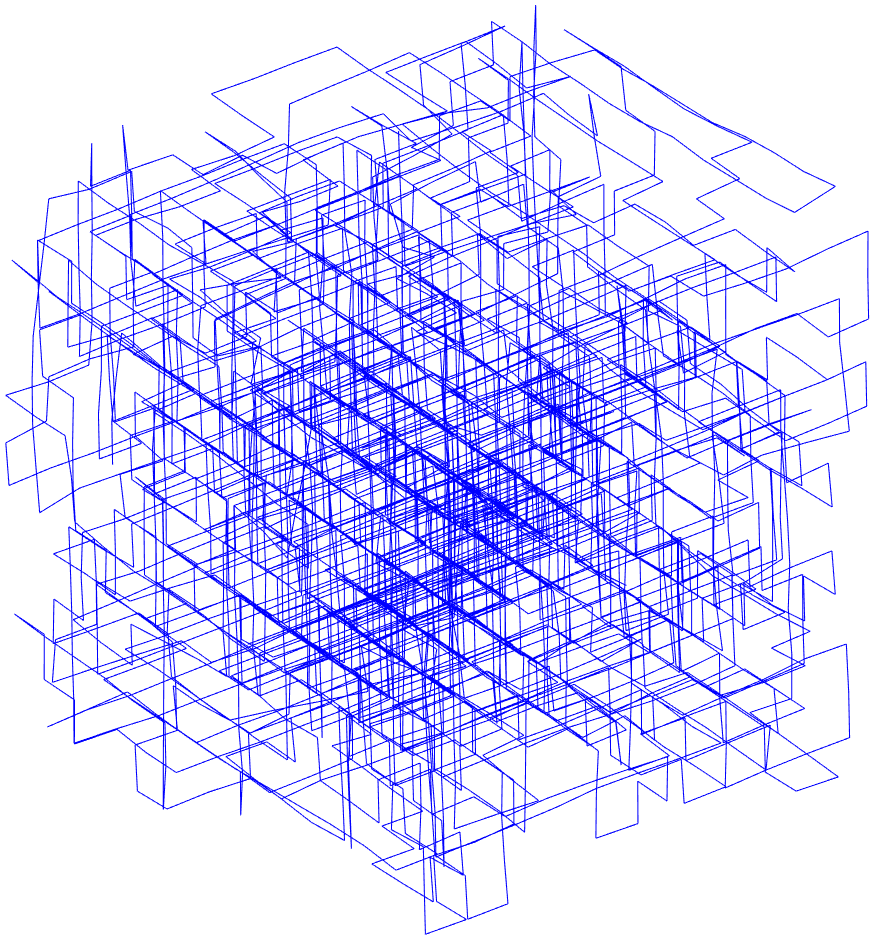
\includegraphics[width=0.175\textwidth]{figures/cube_tests/cube.png}
	\caption{A {\sf\small Cube} dataset has $12\times12\times12$ grids of side length of $1$ m, $3600$ poses, loop closure probability of  $0.1$, an translational RSME of $ 0.02$ m and an angular RSME of $0.02\pi$ rad.}\label{fig::cube}
	\vspace{-0.75em}
\end{figure}

\begin{figure*}[t]
	\centering
	\begin{tabular}{cccc}
		\hspace{-0.5em}\subfloat[][$\ammd$ vs. $\mm$ ]{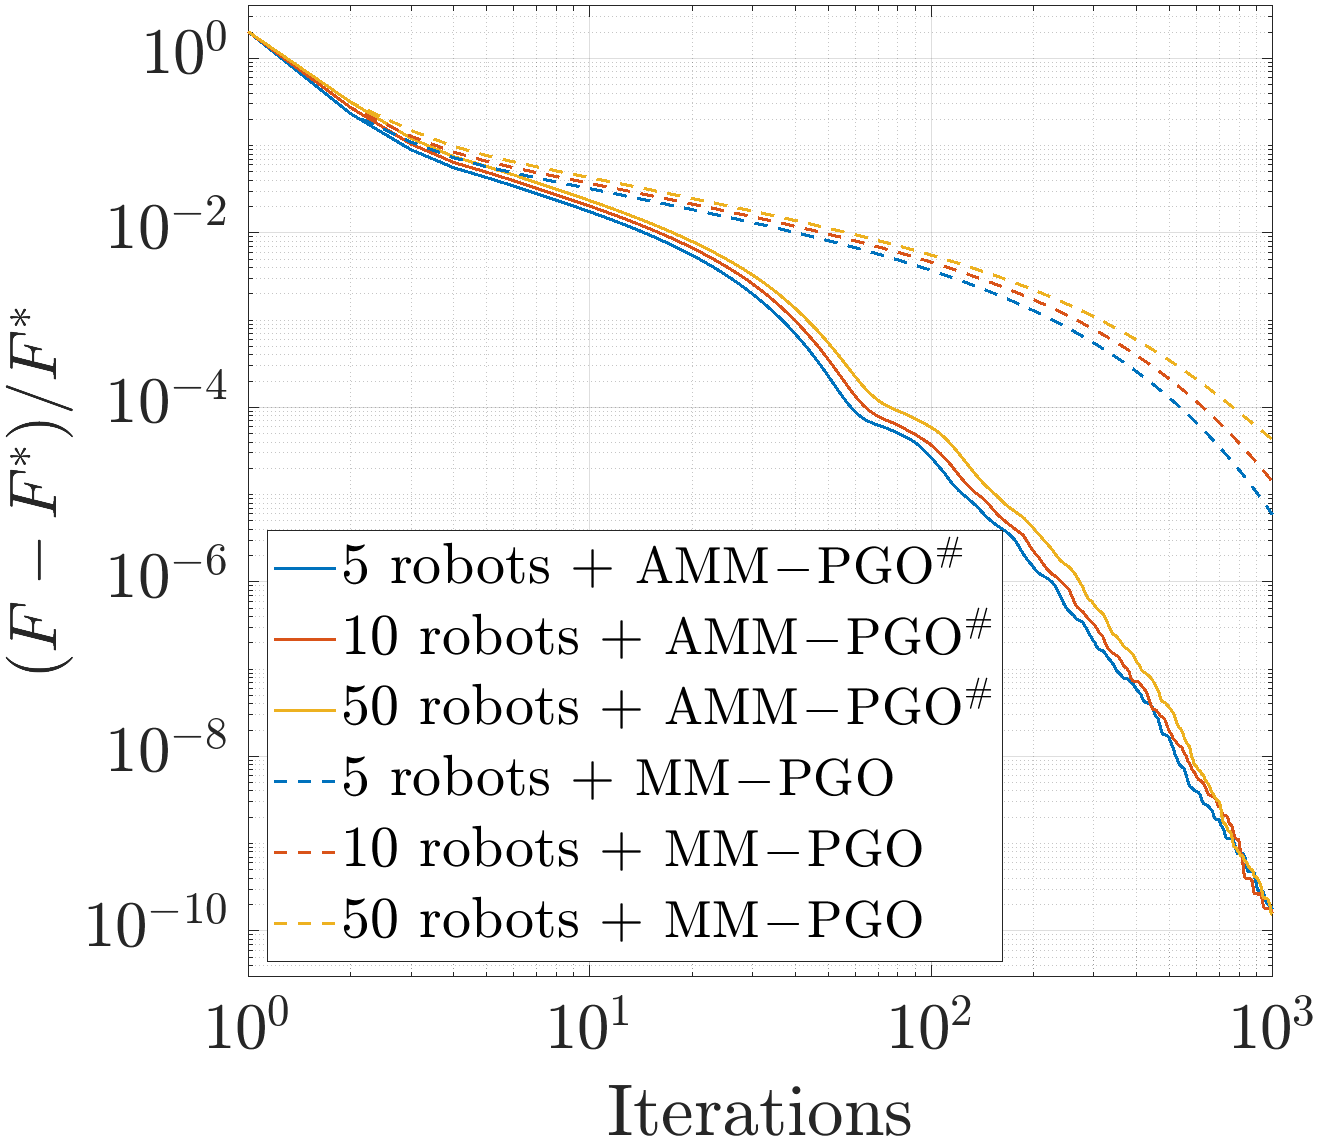
\includegraphics[trim =0mm 0mm 0mm 0mm,width=0.24\textwidth]{figures/cube_tests/rel_none_f.png}} &
		\hspace{-0.6em}\subfloat[][5 robots]{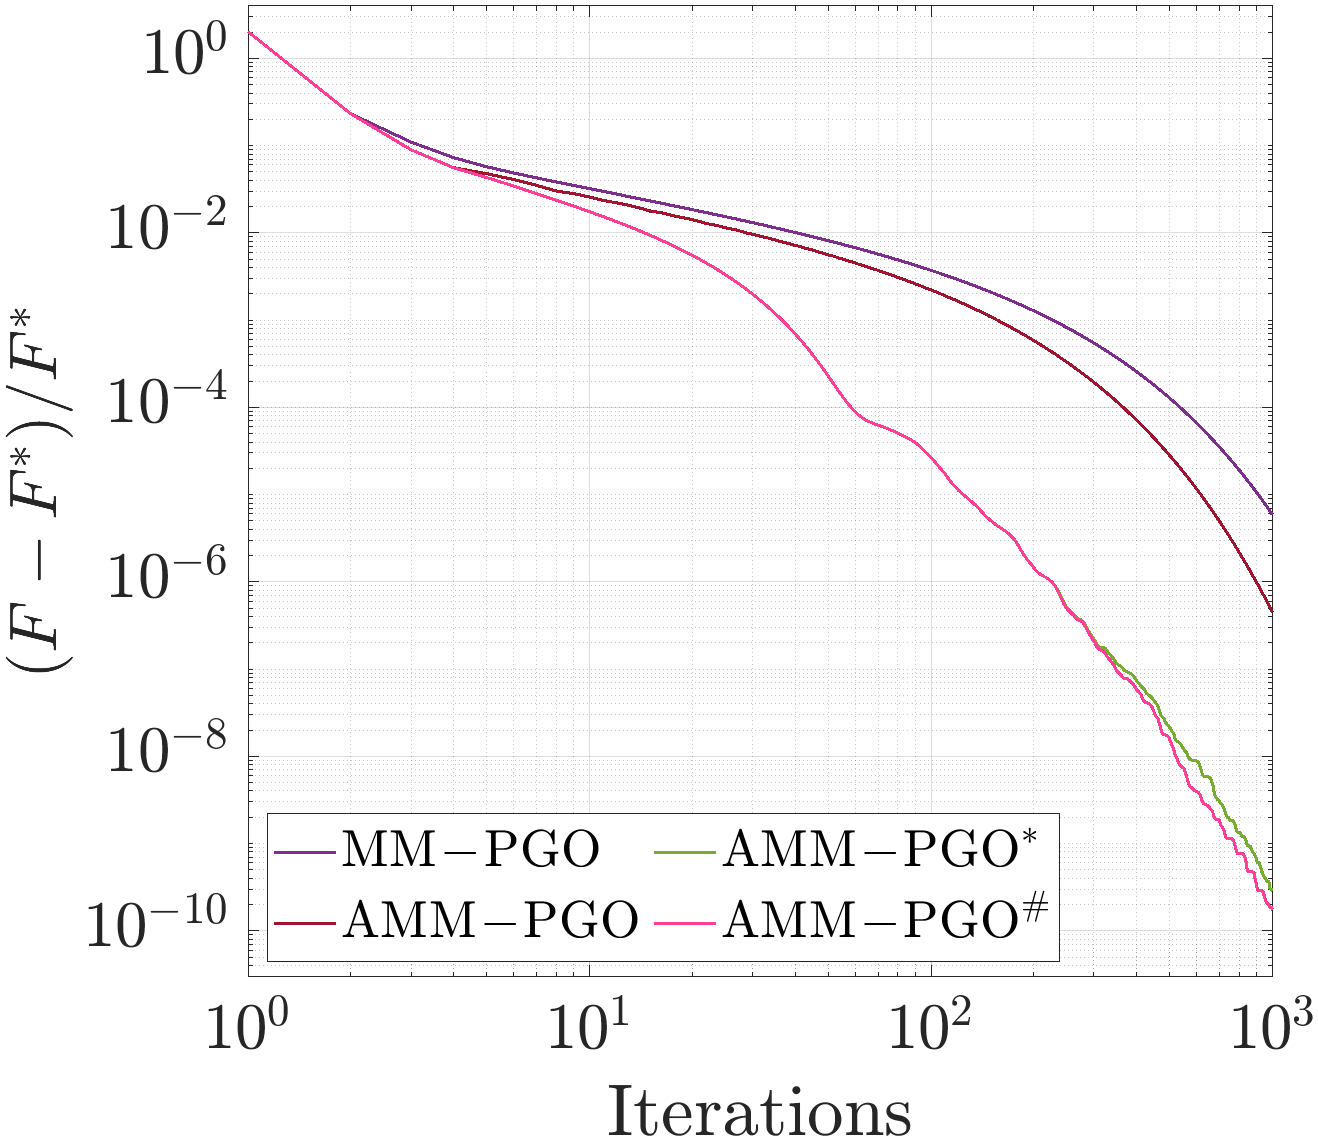
\includegraphics[trim =0mm 0mm 0mm 0mm,width=0.24\textwidth]{figures/cube_tests/rel_none_f_5.png}} &
		\hspace{-0.6em}\subfloat[][10 robots]{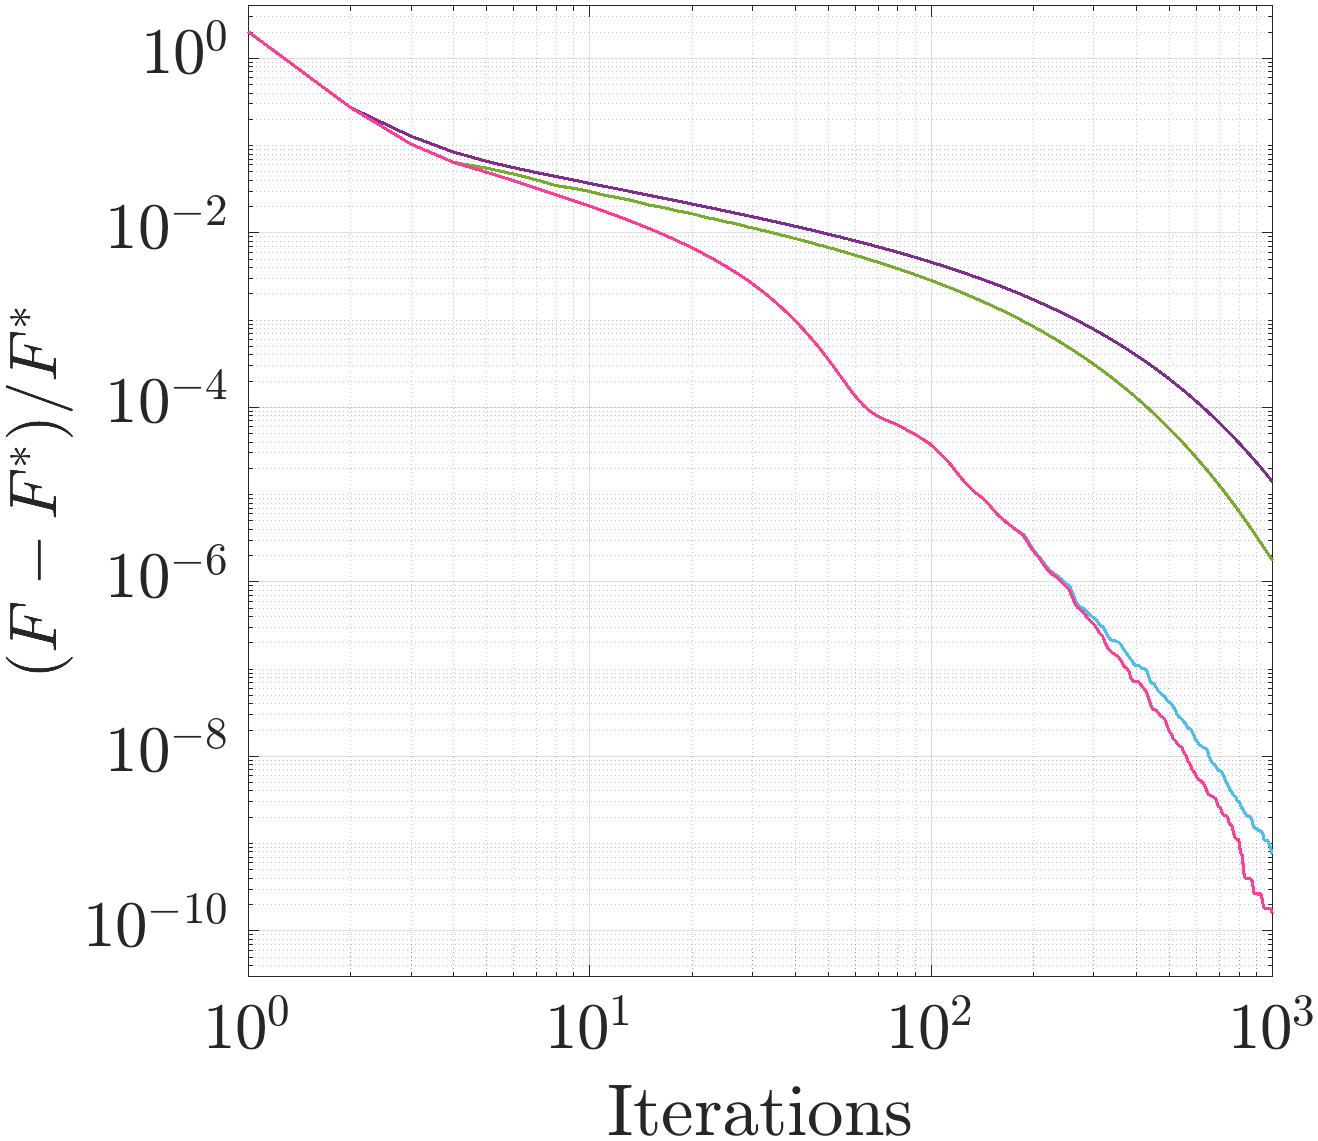
\includegraphics[trim =0mm 0mm 0mm 0mm,width=0.24\textwidth]{figures/cube_tests/rel_none_f_10.png}}&
		\hspace{-0.6em}\subfloat[][50 robots]{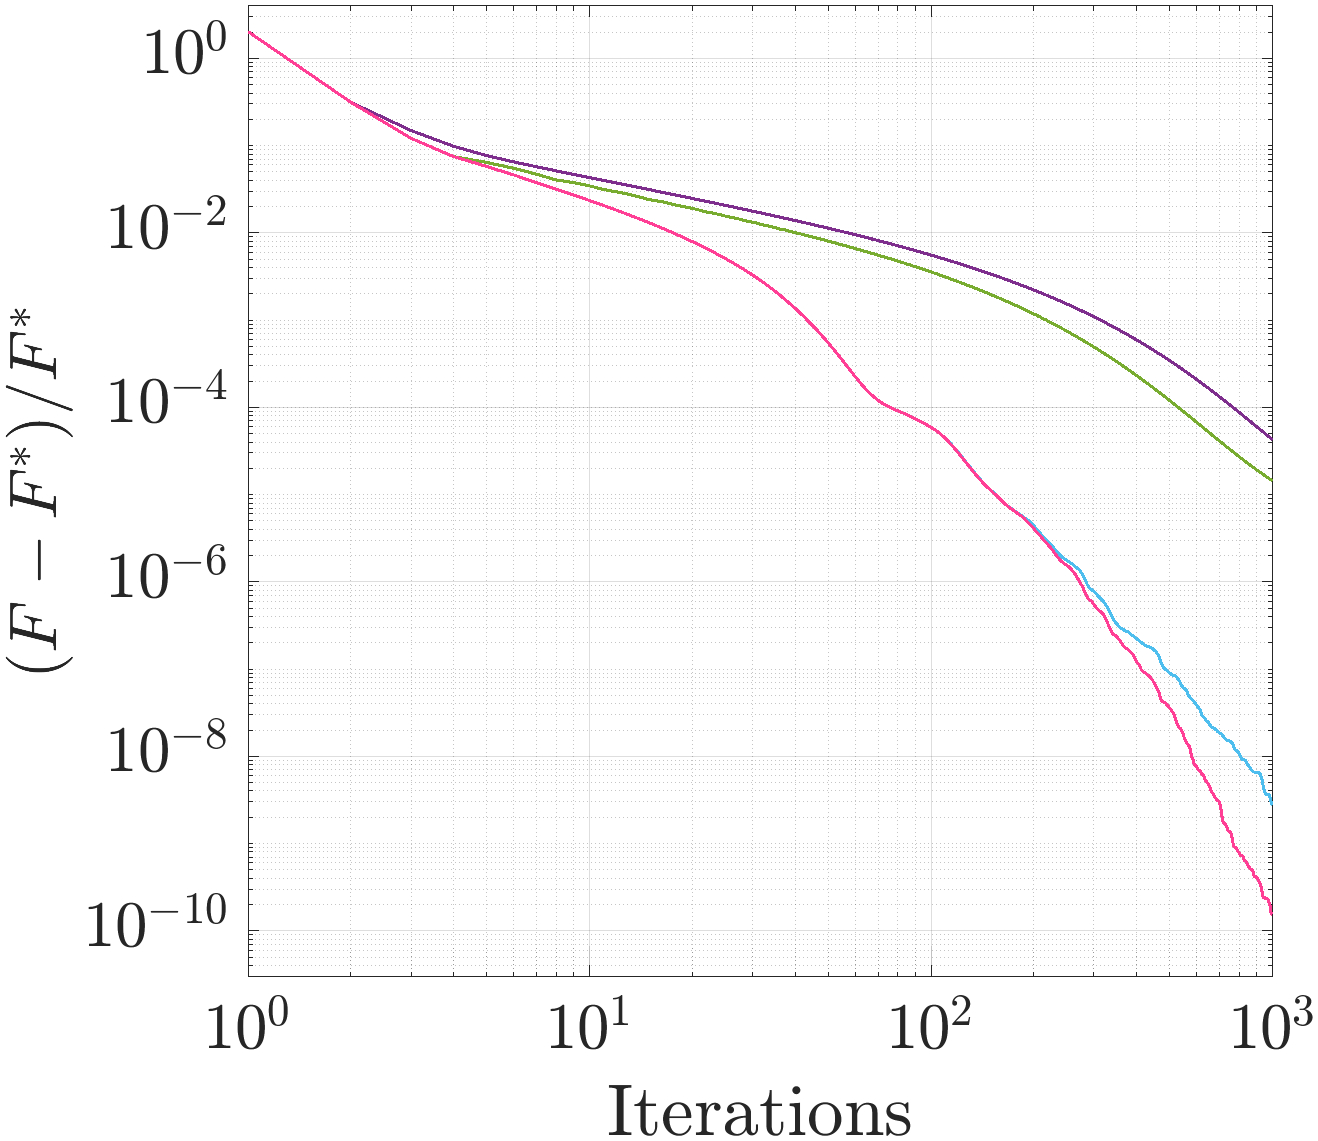
\includegraphics[trim =0mm 0mm 0mm 0mm,width=0.24\textwidth]{figures/cube_tests/rel_none_f_50.png}}
	\end{tabular}
	\caption{The relative suboptimality gaps of  $\mm$, $\ammc$, $\ammd$ and $\amm$ \cite{fan2020mm}  for distributed PGO with the \textbf{trivial loss kernel} on $5$, $10$ and $50$ robots. The results are averaged over $20$  Monte Carlo runs.}\label{fig::cube_f} 
	\vspace{-0.2em}
	
		\begin{tabular}{cccc}
		\hspace{-0.5em}\subfloat[][$\ammd$ vs. $\mm$]{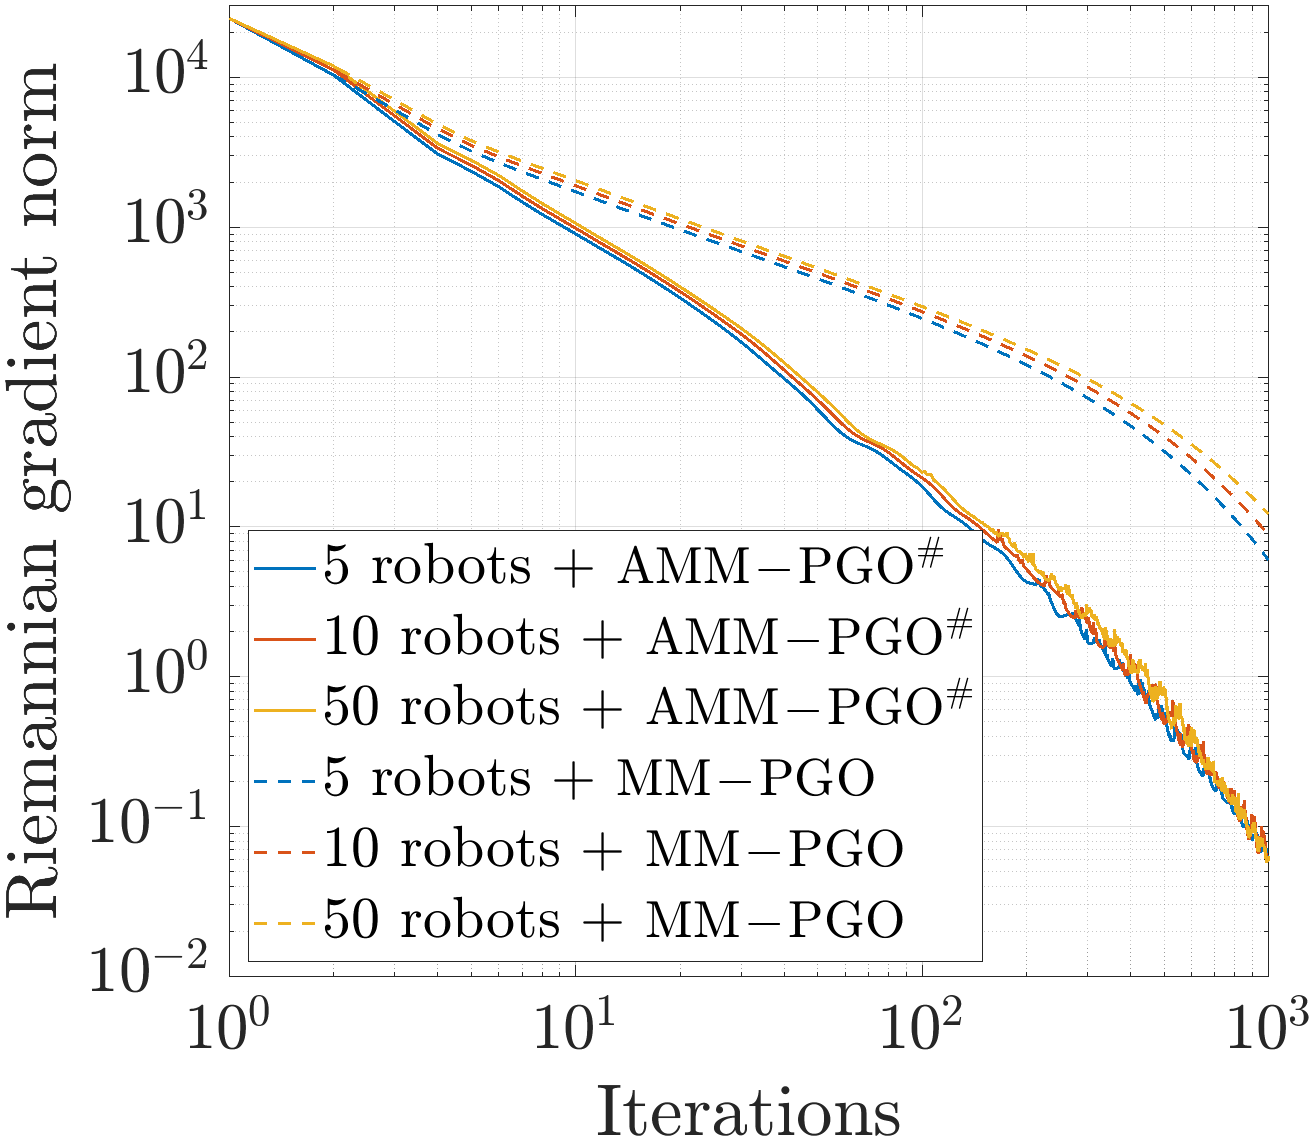
\includegraphics[trim =0mm 0mm 0mm 0mm,width=0.24\textwidth]{figures/cube_tests/rel_none_g.png}} &
		\hspace{-0.6em}\subfloat[][5 robots]{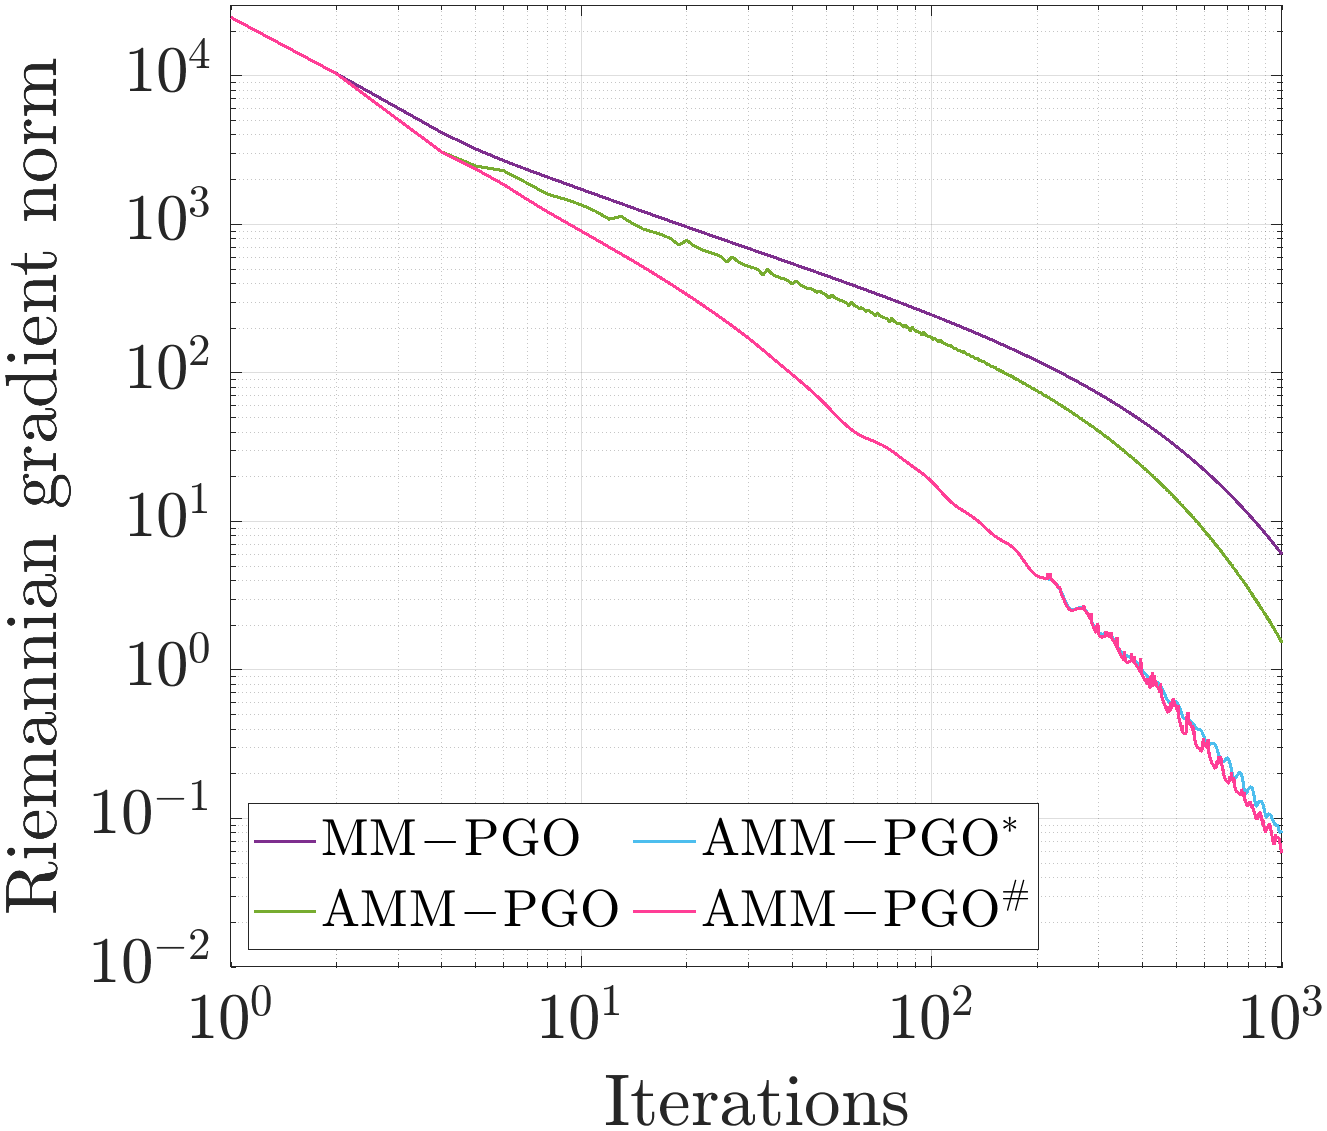
\includegraphics[trim =0mm 0mm 0mm 0mm,width=0.24\textwidth]{figures/cube_tests/rel_none_g_5.png}} &
		\hspace{-0.6em}\subfloat[][10 robots]{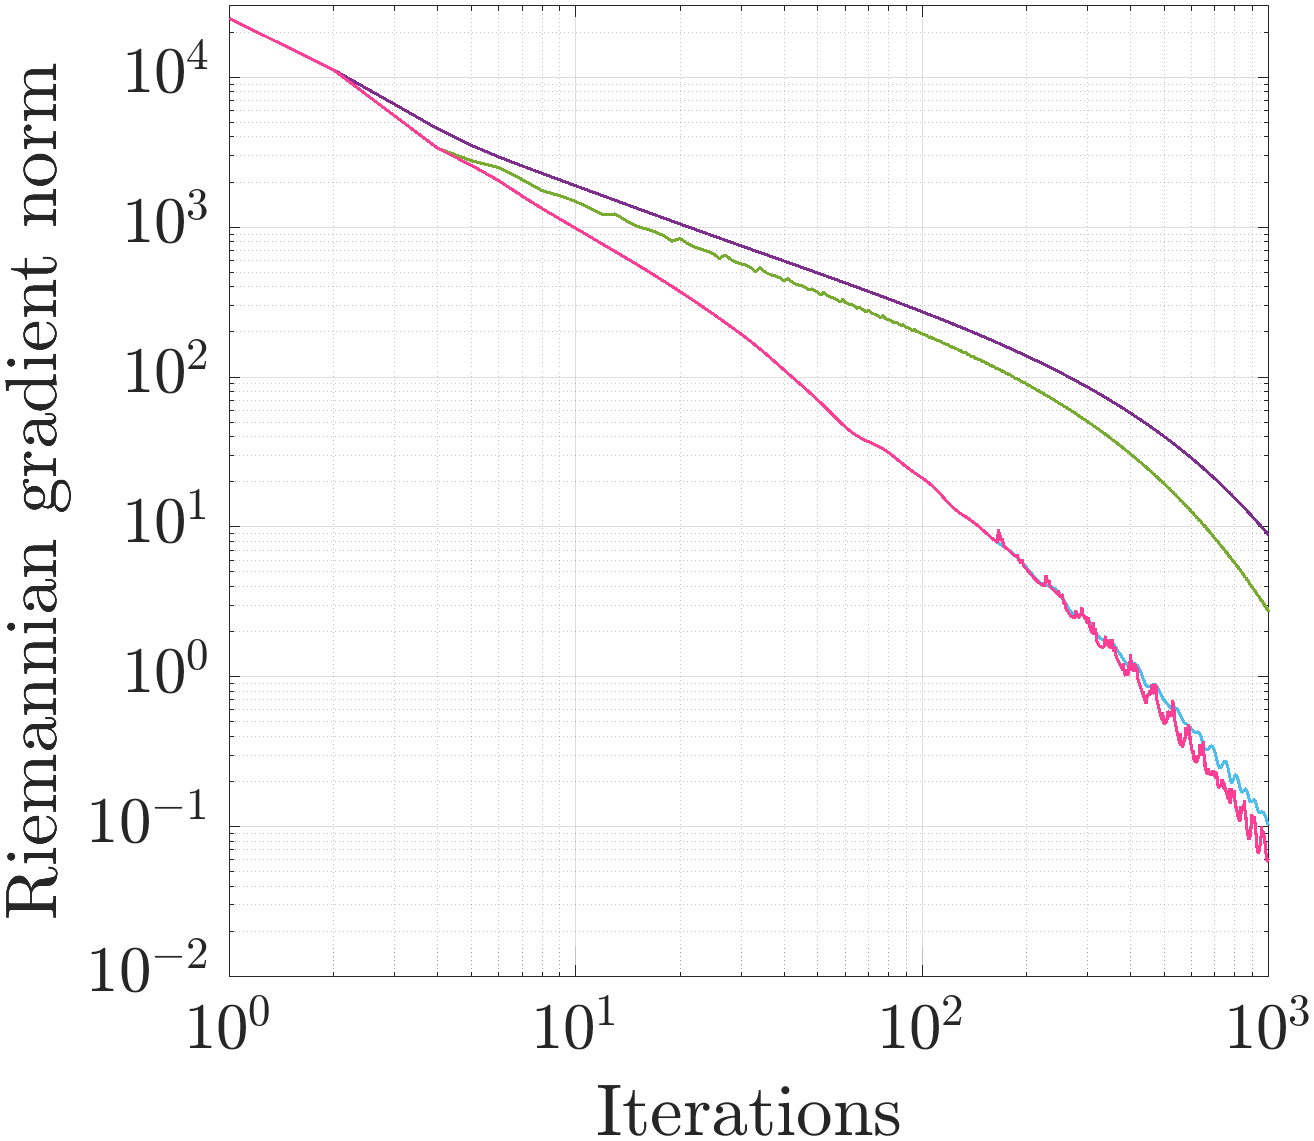
\includegraphics[trim =0mm 0mm 0mm 0mm,width=0.24\textwidth]{figures/cube_tests/rel_none_g_10.png}}&
		\hspace{-0.6em}\subfloat[][50 robots]{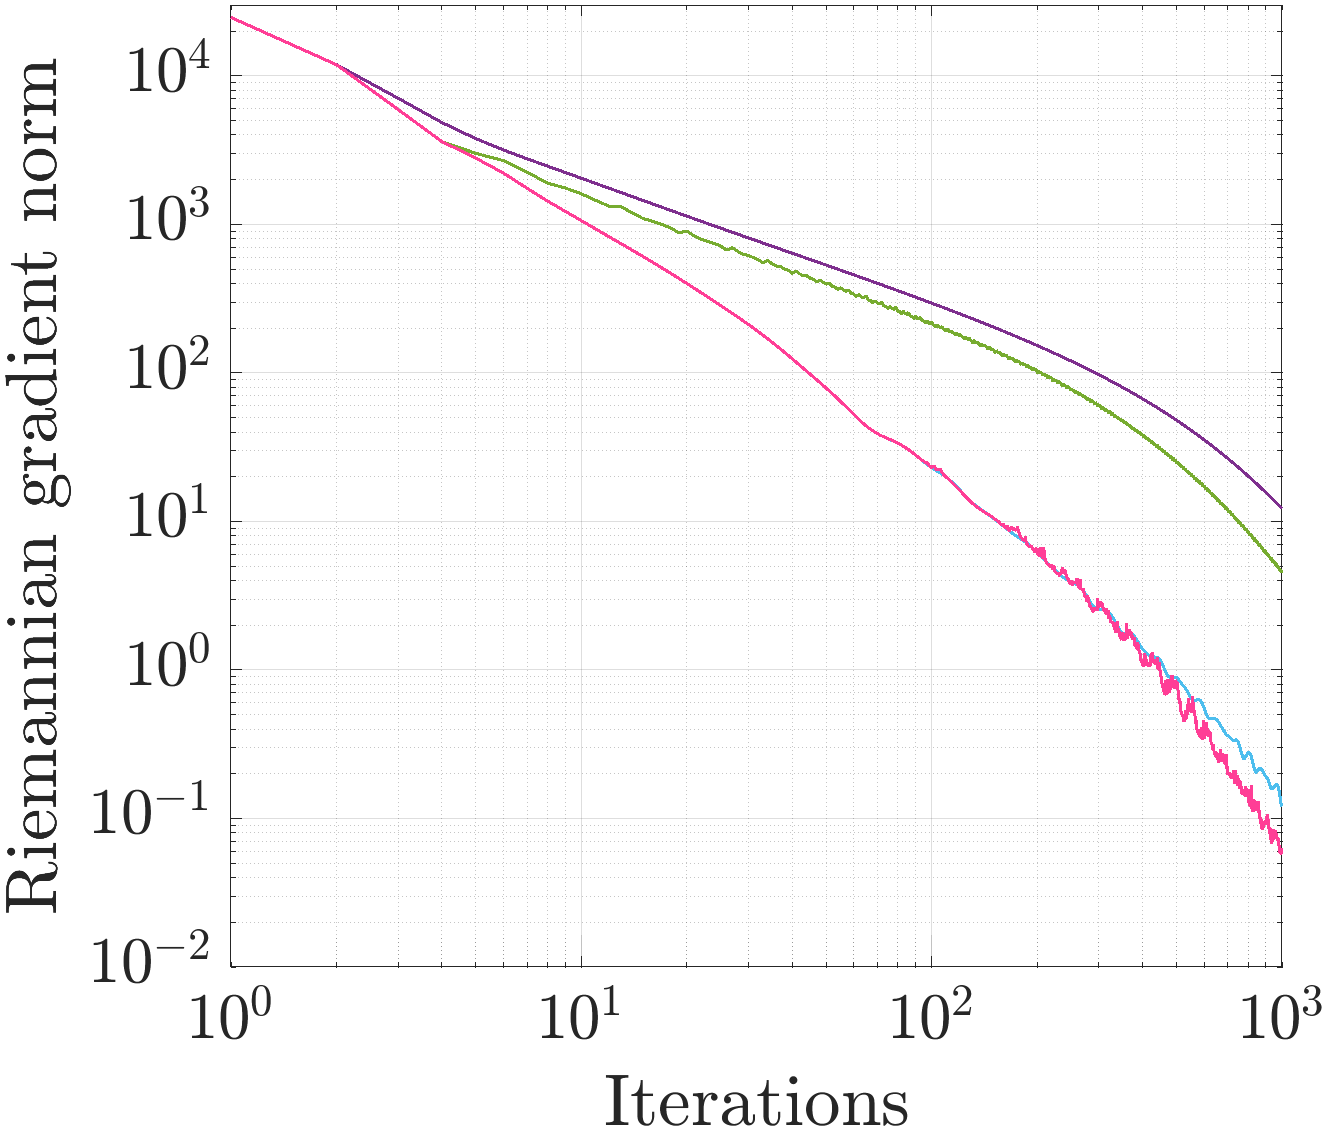
\includegraphics[trim =0mm 0mm 0mm 0mm,width=0.24\textwidth]{figures/cube_tests/rel_none_g_50.png}}
	\end{tabular}
	\caption{The Riemannian gradient norms of  $\mm$, $\ammc$, $\ammd$ and $\amm$ \cite{fan2020mm}  for distributed PGO with the \textbf{trivial loss kernel} on $5$, $10$ and $50$ robots. The results are averaged over $20$  Monte Carlo runs.}\label{fig::cube_g_trivial} 
	\vspace{-1em}
\end{figure*}
	
	\begin{figure*}[t]
		\centering
	\begin{tabular}{cccc}
		\hspace{-0.5em}\subfloat[][$\ammd$ vs. $\mm$]{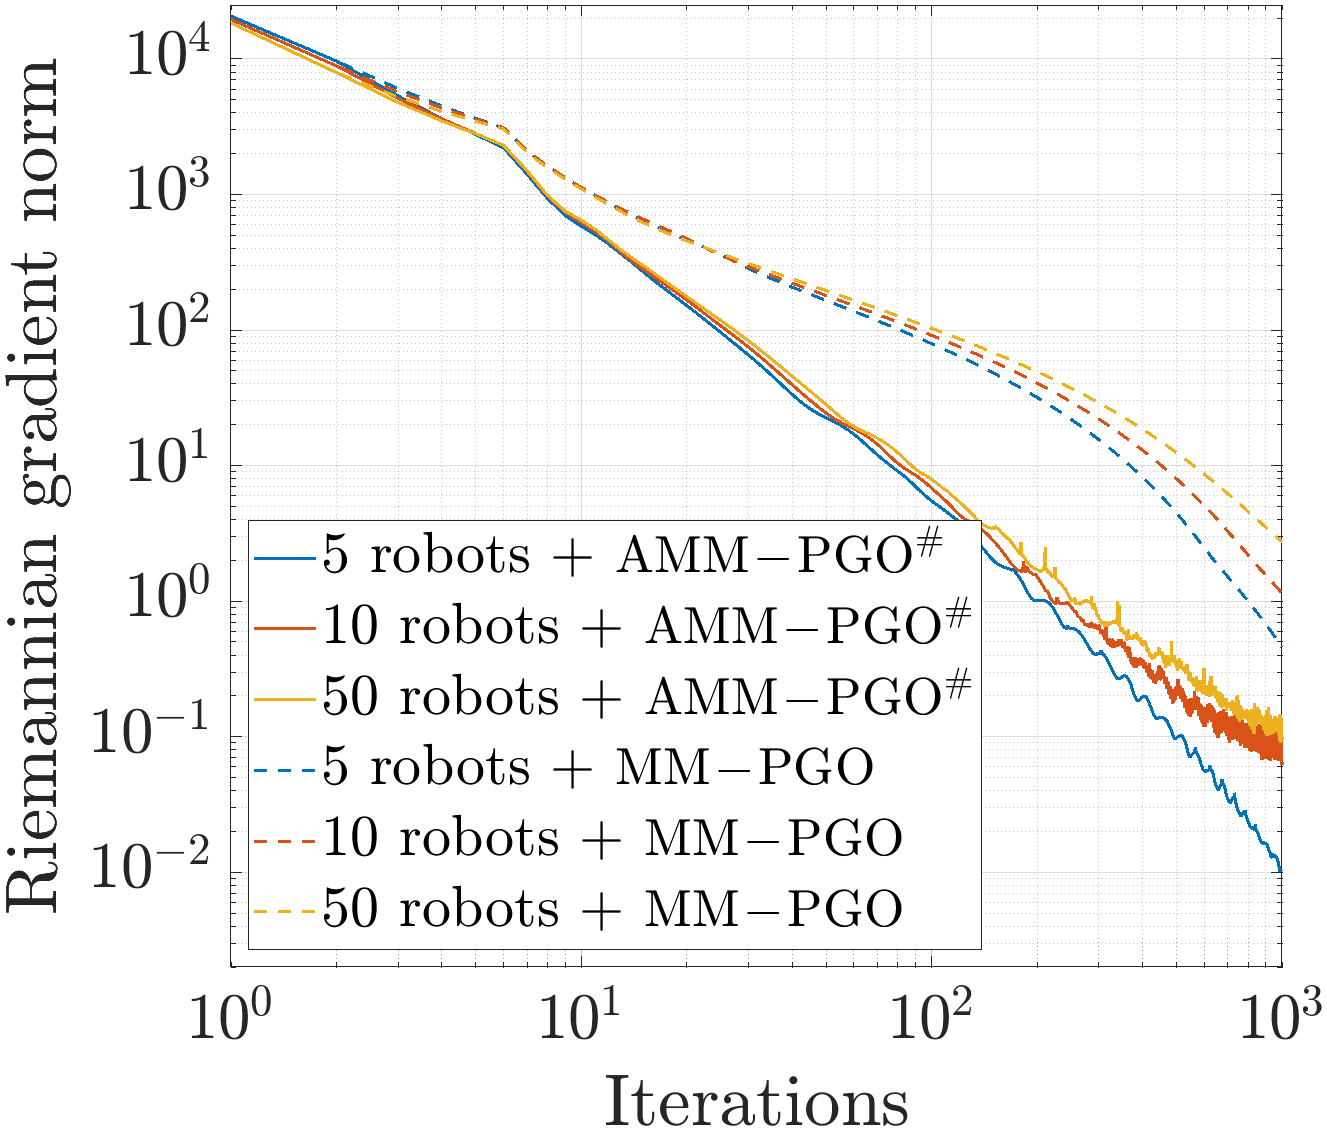
\includegraphics[trim =0mm 0mm 0mm 0mm,width=0.24\textwidth]{figures/cube_tests/rel_huber_g.png}} &
		\hspace{-0.6em}\subfloat[][5 robots]{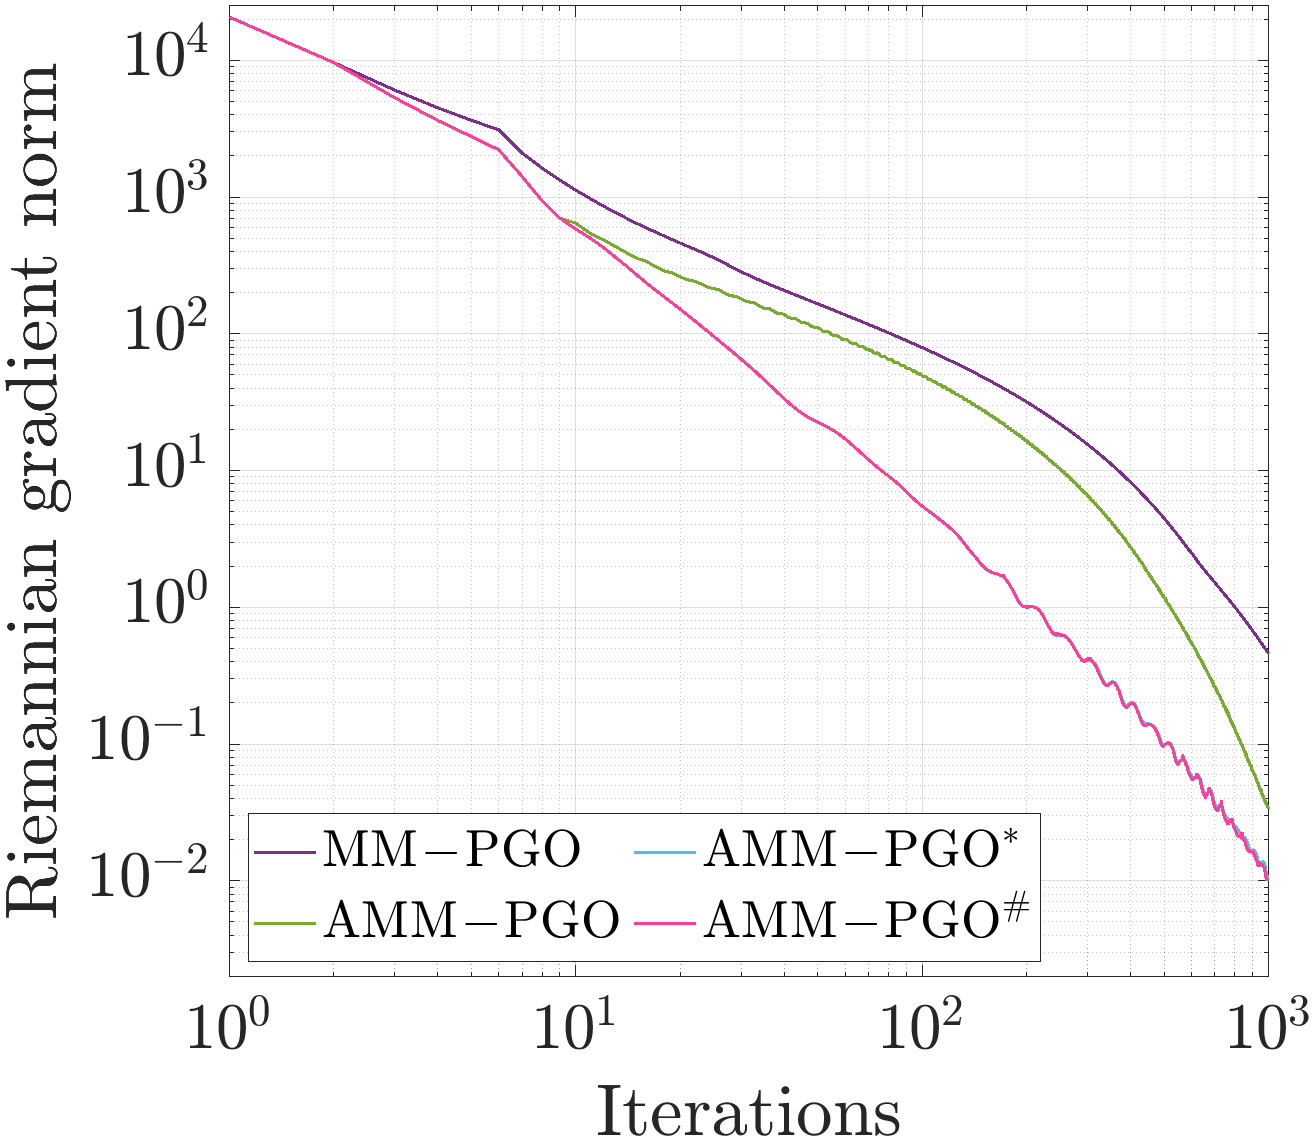
\includegraphics[trim =0mm 0mm 0mm 0mm,width=0.24\textwidth]{figures/cube_tests/rel_huber_g_5.png}} &
		\hspace{-0.6em}\subfloat[][10 robots]{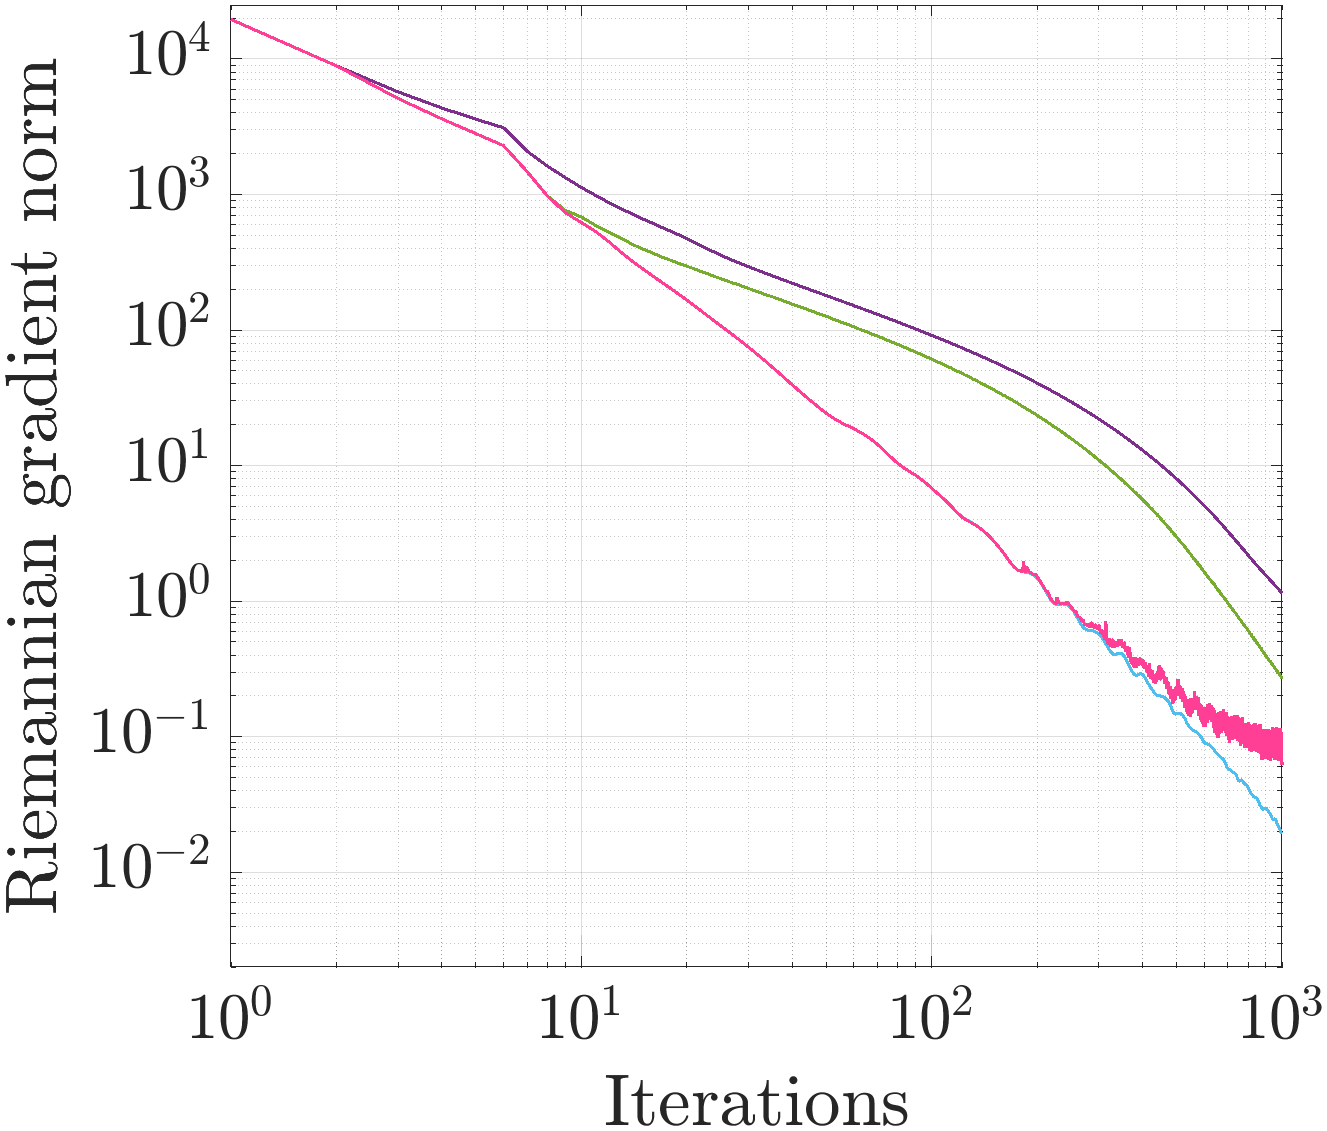
\includegraphics[trim =0mm 0mm 0mm 0mm,width=0.24\textwidth]{figures/cube_tests/rel_huber_g_10.png}}&
		\hspace{-0.6em}\subfloat[][50 robots]{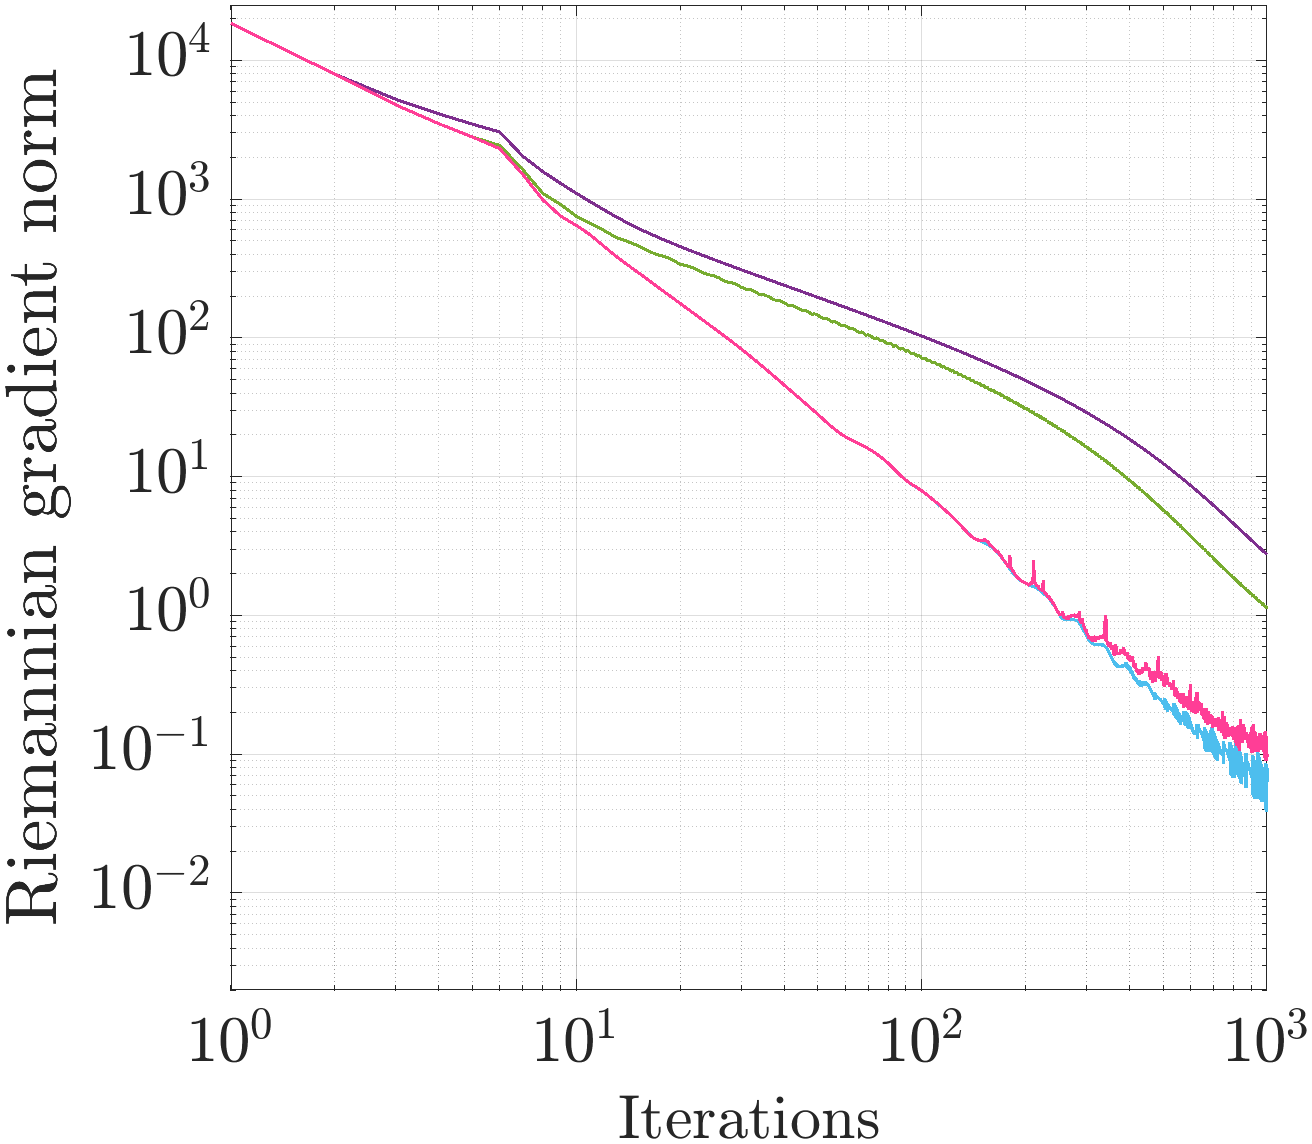
\includegraphics[trim =0mm 0mm 0mm 0mm,width=0.24\textwidth]{figures/cube_tests/rel_huber_g_50.png}}
	\end{tabular}
	\caption{The Riemannian gradient norms of  $\mm$, $\ammc$, $\ammd$ and $\amm$ \cite{fan2020mm}  for distributed PGO with the \textbf{Huber loss kernel} on $5$, $10$ and $50$ robots. The results are averaged over $20$  Monte Carlo runs.}\label{fig::cube_g_huber} 
	\vspace{-0.2em}

	\begin{tabular}{cccc}
		\hspace{-0.5em}\subfloat[][$\ammd$ vs. $\mm$]{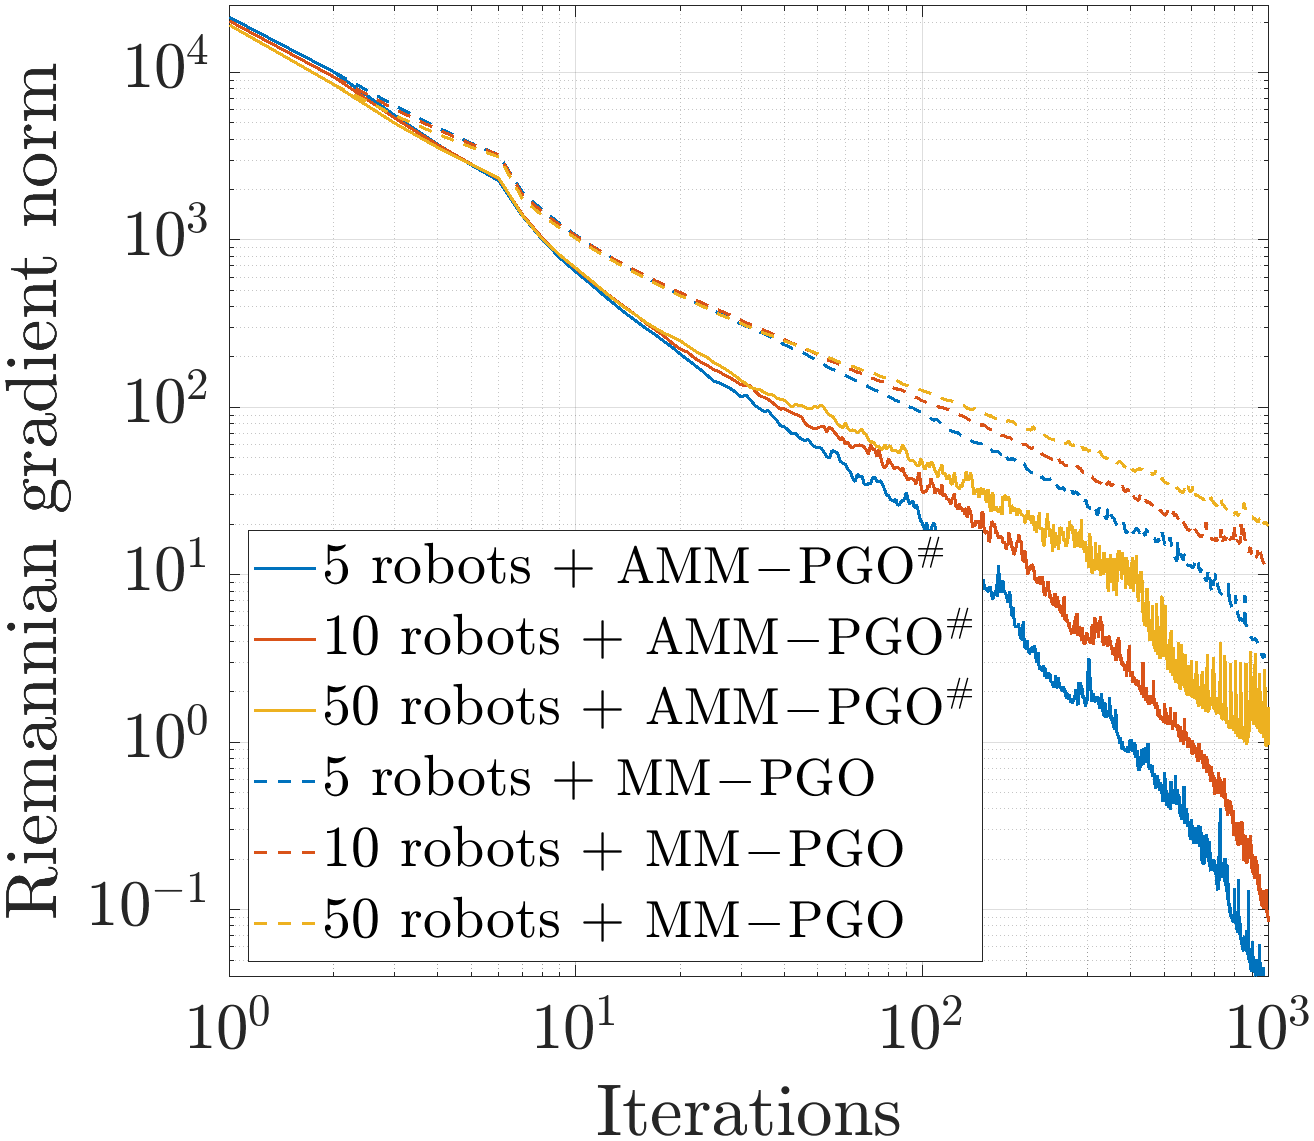
\includegraphics[trim =0mm 0mm 0mm 0mm,width=0.24\textwidth]{figures/cube_tests/rel_welsch_g.png}} &
		\hspace{-0.6em}\subfloat[][5 robots]{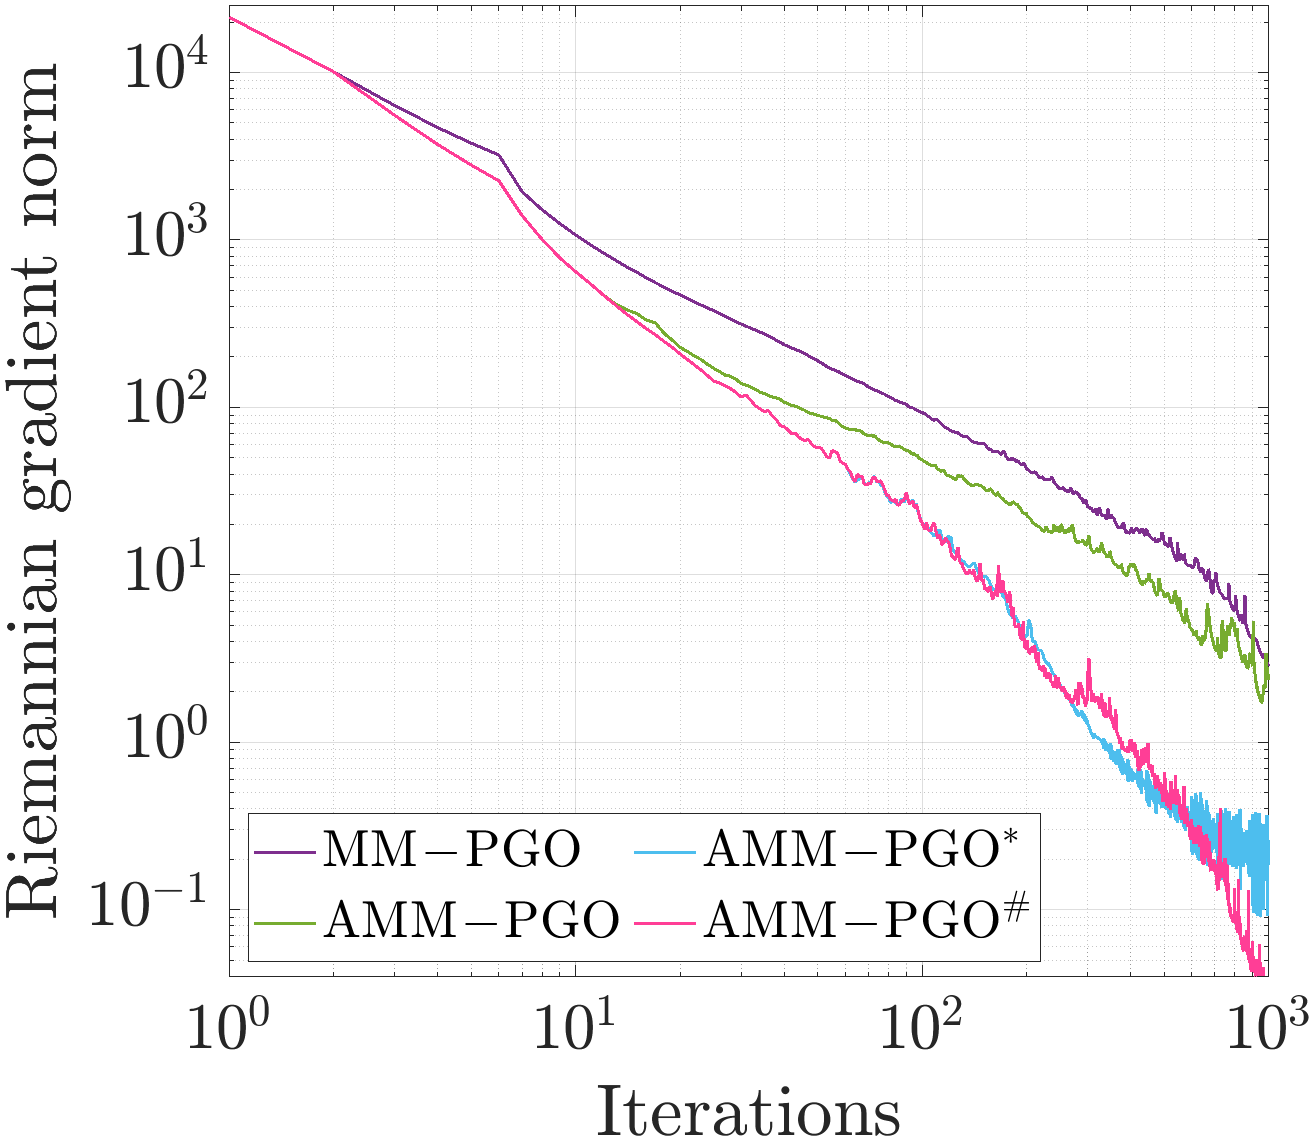
\includegraphics[trim =0mm 0mm 0mm 0mm,width=0.24\textwidth]{figures/cube_tests/rel_welsch_g_5.png}} &
		\hspace{-0.6em}\subfloat[][10 robots]{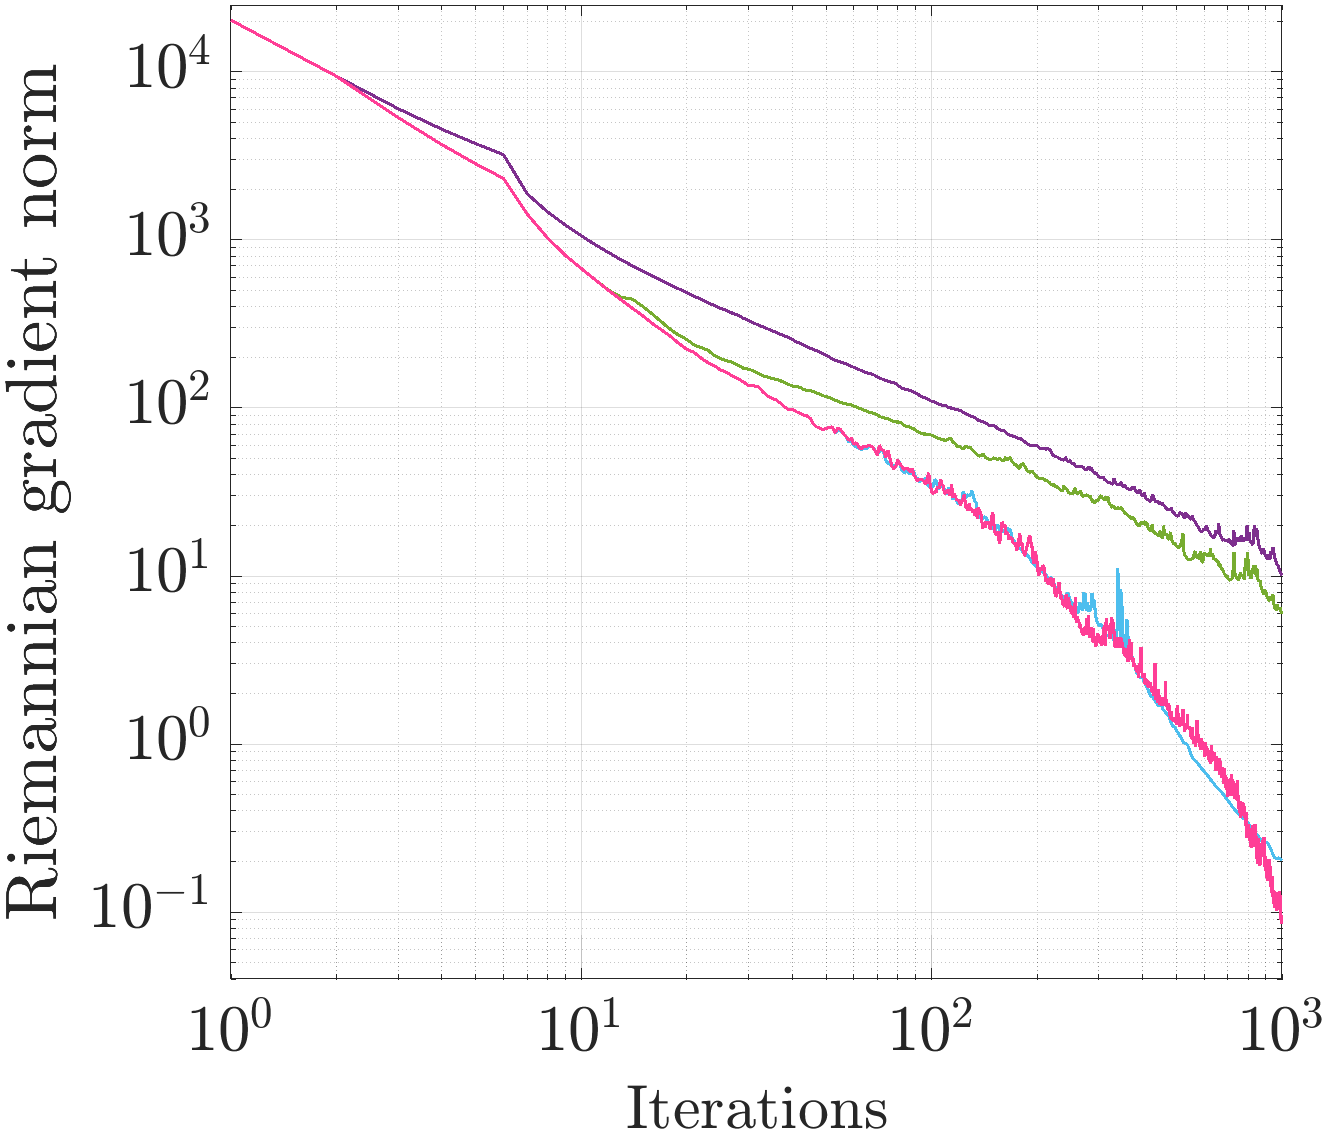
\includegraphics[trim =0mm 0mm 0mm 0mm,width=0.24\textwidth]{figures/cube_tests/rel_welsch_g_10.png}}&
		\hspace{-0.6em}\subfloat[][50 robots]{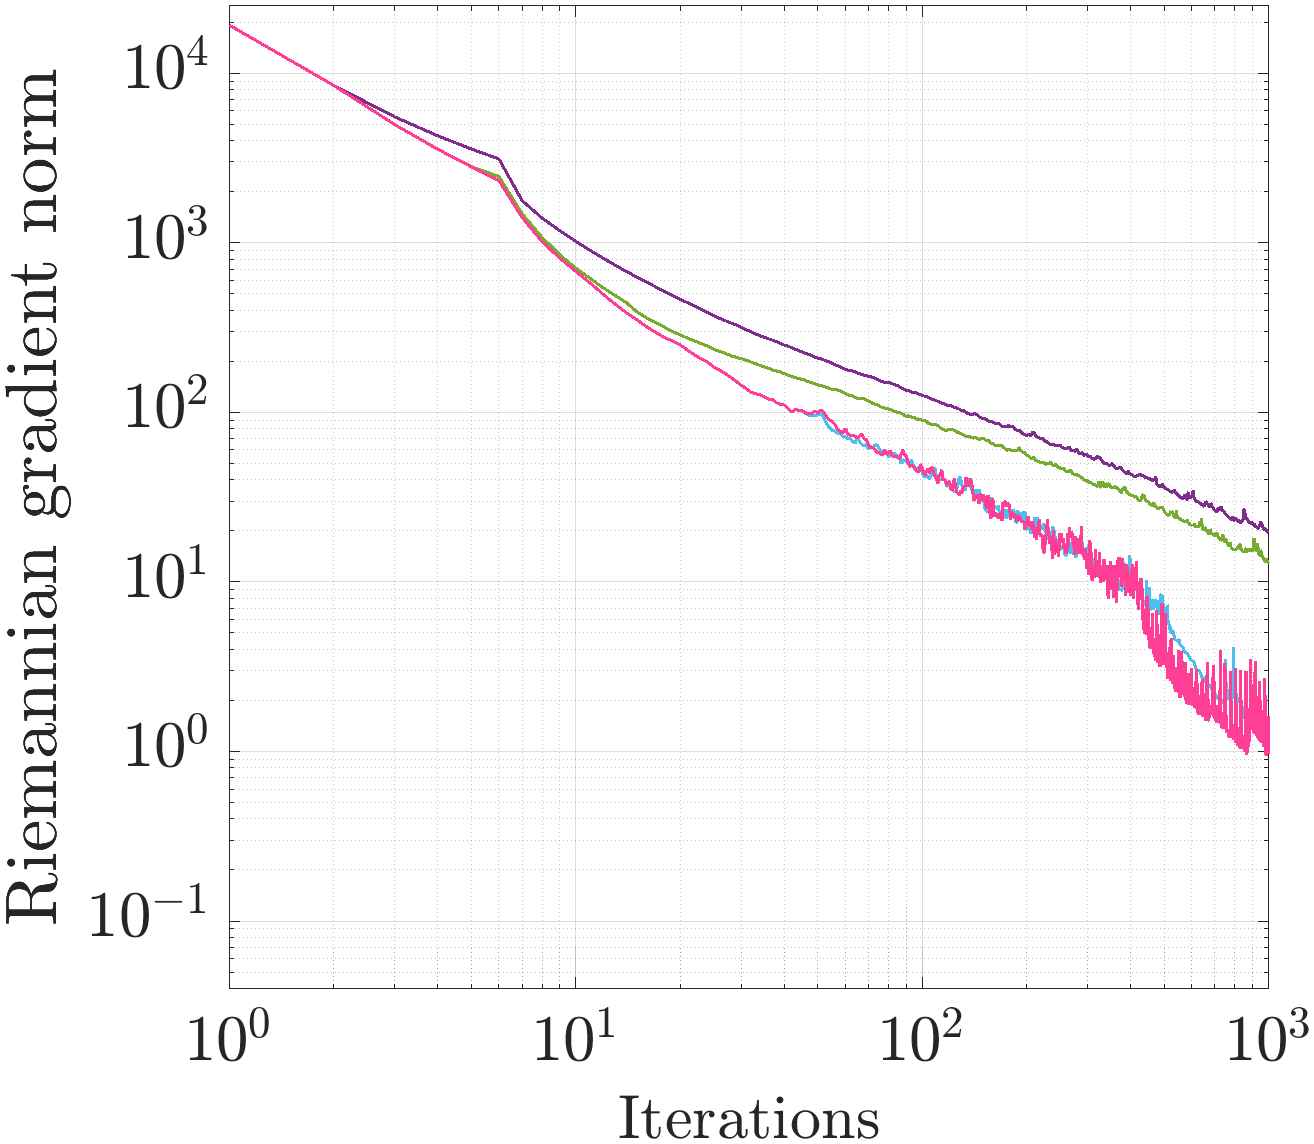
\includegraphics[trim =0mm 0mm 0mm 0mm,width=0.24\textwidth]{figures/cube_tests/rel_welsch_g_50.png}}
	\end{tabular}
	\caption{The Riemannian gradient norms of  $\mm$, $\ammc$, $\ammd$ and $\amm$ \cite{fan2020mm}  for distributed PGO with the \textbf{Welsch loss kernel} on $5$, $10$ and $50$ robots. The results are averaged over $20$  Monte Carlo runs.}\label{fig::cube_g_gm}
	\vspace{-1em}
\end{figure*}


In this section, we test and evaluate our MM methods for distributed PGO on $20$ simulated \textsf{\small Cube} datasets (see \cref{fig::cube})  with $5$, $10$ and $50$ robots. In the experiment, a simulated {\sf\small Cube} dataset has $12 \times 12 \times 12$ cube grids with $1$ m side length, a path of $3600$ poses along the rectilinear edge of the cube grid, odometric measurements between all the pairs of sequential poses, and loop-closure measurements between nearby but non-sequential poses that are randomly available with a probability of $0.1$. We generate the odometric and loop-closure measurements according to the noise models in \cite{rosen2016se} with an expected translational RMSE  of $0.02$ m and an expected angular RMSE of $0.02\pi$ rad. The centralized chordal initialization \cite{carlone2015initialization} is implemented such that distributed PGO with different number of robots have the same initial estimate. The maximum number of iterations is $1000$. 



We evaluate the convergence of $\mm$, $\ammc$ and $\ammd$ in terms of the relative suboptimality gap and Riemannian gradient norm. For reference, we also make comparisons against $\amm$ \cite{fan2020mm}. Note that $\amm$ is the original accelerated MM method for distributed PGO whose adaptive restart scheme is conservative and might  prohibit Nesterov's acceleration.

\textbf{Relative Suboptimality Gap.} We implement the certifiably-correct $\sesync$ \cite{rosen2016se} to get the globally optimal objective value $F^*$  of distributed PGO with the trivial loss kernel (\cref{example::trivial}), making it possible to compute the relative suboptimality gap $(F-F^*)/F^*$ where $F$ is the objective value for each iteration. The results are in \cref{fig::cube_f}.

\textbf{Riemannian Gradient Norm.}  We also compute the Riemannian gradient norm of distributed PGO with the trivial, Huber  and Welsch loss kernels in \cref{example::huber,example::GM,example::trivial} for evaluation. Note that it is difficult to find globally optimal solutions to distributed PGO if Huber and Welsch loss kernels are used. The results are in \cref{fig::cube_g_huber,fig::cube_g_gm,fig::cube_g_trivial}.



In \cref{fig::cube_g_gm,fig::cube_g_huber,fig::cube_f,fig::cube_g_trivial}, it can be seen that $\mm$, $\ammc$, $\ammd$ and $\amm$ have a faster convergence if the number of robots (nodes) decreases. This is expected since $G(X|X^{(k)})$ and $H(X|X^{(k)})$ in \cref{eq::G,eq::lG} result in tighter approximations for distributed PGO with fewer robots (nodes). In addition, \cref{fig::cube_g_gm,fig::cube_g_huber,fig::cube_g_trivial} suggest that the convergence rate of $\mm$, $\ammc$, $\ammd$ and $\amm$ also relies on the type of loss kernels. Nevertheless, $\ammc$, $\ammd$ and $\amm$ accelerated by Nesterov's method outperform  unaccelerated $\mm$  by a large margin for any number of robots and any types of loss kernels, which means that Nesterov's method improves the convergence of distributed PGO. In particular, Figs. \ref{fig::cube_f}(a), \ref{fig::cube_g_trivial}(a), \ref{fig::cube_g_huber}(a), \ref{fig::cube_g_gm}(a) indicate that $\ammd$  with $50$ robot still converges faster than $\mm$ with $5$ robots despite that the later has a much smaller number of robots. Therefore, we conclude that Nesterov's method accelerates the convergence of distributed PGO.



We emphasize the convergence comparisons of Nesterov's accelerated $\ammc$, $\ammd$ and $\amm$ that merely differ from each other by the adaptive restart schemes---$\ammc$ has an additional master node to aggregate information from all the robots (nodes), whereas $\ammd$ and $\amm$ are restricted to one inter-node communication round per iteration among neighboring robots (nodes). Notwithstanding limited local communication, as is shown in \cref{fig::cube_f,fig::cube_g_huber,fig::cube_g_gm}, $\ammd$ has a convergence rate comparable to that of $\ammc$ using a master node while being significantly faster than $\amm$.  {\highlight In particular,  $\ammd$ reduces adaptive restarts by $80\%$ to $95\%$ compared to $\amm$ on the \textsf{\small Cube} datasets}, and thus, is expected to make better use of Nesterov's acceleration. Since $\ammd$ and $\amm$ differ in the adaptive restart schemes, we attribute the faster convergence of $\ammd$ to its redesigned adaptive restart scheme. These results suggest that $\ammd$ is advantageous over other methods for very large-scale distributed PGO where computational and communicational efficiency are equally important.

\vspace{-0.5em}

%\begin{table}[H]
	\centering
	\setlength{\tabcolsep}{0.3em}
	\renewcommand{\arraystretch}{1.2}
	\caption{2D and 3D SLAM benchmark datasets.}\label{table::dataset}
	\begin{tabular}{|P{0.07\textwidth}|P{0.055\textwidth}|P{0.065\textwidth}|P{0.11\textwidth}|P{0.1\textwidth}|}
		\hline			
		\multirow{2}{*}{Dataset} & \multirow{2}{*}{2D/3D} & \multirow{2}{*}{\# Poses} & \multirow{2}{*}{\# Measurements}  & Real-World Dataset \\
		\hline
		\hline
		{\sf ais2klinik} & 2D &15115 & 16727 & \cmark\\
		\hline
		{\sf city} & 2D & 10000 & 20687 & \xmark\\
		\hline
		{\sf CSAIL} & 2D & 1045 & 1172 & \cmark \\
		\hline
		{\sf M3500} & 2D & 3500 & 5453 & \xmark \\
		\hline
		{\sf intel} & 2D & 1728 & 2512 & \cmark\\
		\hline
		{\sf MITb} & 2D & 808 & 827 & \cmark \\
		\hline
		{\sf sphere} & 3D & 2500 & 4949 & \xmark\\
		\hline
		{\sf torus} & 3D & 5000 & 9048 & \xmark\\
		\hline
		{\sf grid} & 3D & 8000 & 22236 & \xmark\\
		\hline
		{\sf garage} & 3D & 1661 & 6275 & \cmark\\
		\hline
		{\sf cubicle} & 3D & 5750 & 16869 & \cmark\\
		\hline
		{\sf rim} & 3D & 10195 & 29743 & \cmark\\
		\hline
	\end{tabular}
\vspace{-1em}
\end{table}



\vspace{-0.5em}
\subsection{Benchmark Datasets}\label{subsection::experiment::benchmark}
In this section, we evaluate our MM methods ($\mm$, $\ammc$ and $\ammd$) for distributed PGO on a number of 2D and 3D SLAM benchmark datasets \cite{rosen2016se} (see \datasetinfo). We use the trivial loss kernel and there are no outliers such that the globally optimal solution can be exactly computed with $\sesync$ \cite{rosen2016se}. For each dataset, we also make comparisons against $\sesync$ \cite{rosen2016se}, distributed Gauss-Seidel ($\dgs$) \cite{choudhary2017distributed} and the Riemannian block coordinate descent ($\rbcd$) \cite{tian2019distributed} method\footnote{$\rbcd$ \cite{tian2019distributed} solves the lifted problem which usually results in slightly smaller objective values than the original problem.}, all of which are the state-of-the-art algorithms for centralized and distributed PGO. The $\sesync$ and $\dgs$ methods use the recommended settings in \cite{choudhary2017distributed,rosen2016se}. We implement two Nesterov's accelerated variants of $\rbcd$  \cite{tian2019distributed}, i.e., one with greedy selection rule and adaptive restart ($\rbcdc$) and the other with uniform selection rule and fixed restart ($\rbcdd$)\footnote{In the experiments, we run $\rbcdd$ \cite{tian2019distributed} with fixed restart frequencies of 30, 50 and 100 iterations for each dataset and report the best results.}. As mentioned before, $\ammc$ and $\ammd$ can take at most one iteration when updating $\Xakp$ using \cref{eq::GYak,eq::xG}, which is similar to $\rbcdc$ and $\rbcdd$. An overview of the aforementioned methods is given in \cref{table::cmp_method}.

\begin{table}
	\centering
		\renewcommand{\arraystretch}{1.2}
	\setlength{\tabcolsep}{0.3em}
	\caption{An overview of the state-of-the-art algorithms for distributed and centralized PGO. Note that $\ammc$ and $\rbcdc$ require a master node for distributed PGO, and $\ammd$  is the only accelerated method with provable convergence for distributed PGO without master node.
	}\label{table::cmp_method}
	\begin{tabular}{|P{0.125\textwidth}|P{0.07\textwidth}|P{0.075\textwidth}|P{0.085\textwidth}|P{0.075\textwidth}|}
		\hline			
%		\multirow{2}{*}{Method} &\multirow{2}{*}{Distributed} & \multirow{2}{*}{Accelerated}  &Master Node Required & \multirow{2}{*}{Converged}\\
		{Method} &{Distributed} & {Accelerated}  &Masterless & {Converged}\\
		\hline
		\hline
		$\sesync$\cite{rosen2016se}& \xmark & N/A & N/A & \cmark \\
		\hline
		$\dgs$\cite{choudhary2017distributed} &\cmark & \xmark & \cmark & \xmark \\
		\hline
		$\rbcdc$\cite{tian2019distributed}&\cmark& \cmark & \xmark & \cmark\\
		\hline
		$\rbcdd$\cite{tian2019distributed}&\cmark & \cmark & \cmark & \xmark\\
		\hline
		$\mm$ & \cmark &\xmark & \cmark & \cmark \\
		\hline
		$\ammc$&\cmark & \cmark & \xmark & \cmark\\
		\hline
		$\ammd$&\cmark & \cmark & \cmark & \cmark \\
		\hline
	\end{tabular}
\end{table}

\begin{table*}[t]
	\renewcommand{\arraystretch}{1.22}
		\setlength{\tabcolsep}{0.25em}
	\centering
	\caption{Results of distributed PGO on 2D and 3D SLAM benchmark datasets (see \datasetinfo). The distributed PGO has 10 robots  and is initialized with distributed Nesterov's accelerated chordal initialization \cite{fan2020mm}. We report the objective values of each method with 100, 250 and 1000 iterations. $F^{(\sk)}$ and $F^*$ are the objective value at iteration $\sk$ and globally optimal objective value, respectively. The best results are colored in {\color{red}red} and the second best in {\color{blue}blue} if no methods tie for the best.}	\label{table::comp}
	\begin{tabular}{|c||c|c||c|c|c||c|c|c|c|}
		\hline
		\multirow{3}{*}{Dataset}&\multirow{3}{*}{$F^{(0)}$} &\multirow{3}{*}{$F^{*}$} &\multirow{3}{*}{\;$\sk$\;}& \multicolumn{6}{c|}{$F^{(\sk)}$}\\
		\cline{5-10}
		& & & & \multicolumn{2}{c||}{Methods w/ Master Node} & \multicolumn{4}{c|}{Methods w/o Master Node}\\
		\cline{5-10}
		& & & & \;$\ammc$\;  & $\rbcdc$ \cite{tian2019distributed} & $\;\;\;\mm\;\;\;$  & \;$\ammd$\;  & $\;\;\;\dgs$ \cite{choudhary2017distributed} $\;$ & {$\rbcdd$ \cite{tian2019distributed}}  \\
		\hline
    \multicolumn{10}{|c|}{{2D SLAM Benchmark Datasets}}\\
		\hline
		\multirow{3}{*}{\sf ais2klinik} &\multirow{3}{*}{$3.8375\times 10^2$} &\multirow{3}{*}{$1.8850\times 10^2$}
    &100 & {\color{blue}$2.0372\times 10^{2}$} &$2.1079\times 10^{2}$ & $2.1914\times 10^{2}$ & {\color{red}$2.0371\times 10^{2}$} & $8.4701\times 10^{2}$ & $2.1715\times 10^{2}$  \\
		\cline{4-10}
		& &
    &250 & {\color{blue}$1.9447\times 10^{2}$} &$2.0077\times 10^{2}$ & $2.1371\times 10^{2}$ & {\color{red}$1.9446\times 10^{2}$} & $9.1623\times 10^{1}$ & $2.1084\times 10^{2}$  \\
		\cline{4-10}
		& &
    &1000& {\color{blue}$1.8973\times 10^{2}$} &$1.9074\times 10^{2}$ & $2.0585\times 10^{2}$ & {\color{red}$1.8936\times 10^{2}$} & $3.8968\times 10^{2}$ & $2.0253\times 10^{2}$  \\
		\hline
    \multirow{3}{*}{\sf city} &\multirow{3}{*}{$7.0404\times 10^2$} &\multirow{3}{*}{$6.3862\times 10^2$}
    &100 &\color{ao}$6.4327\times 10^2$ & $6.5138\times 10^2$ &$6.5061\times 10^2$ &\color{ao}$6.4327\times10^{2}$ &$7.7745\times10^{2}$ & $6.5396\times 10^2$ \\
		\cline{4-10}
    & &
    &250 &\color{ao}$6.3899\times 10^2$ & $6.4732\times 10^2$ &$6.4850\times 10^2$ &\color{ao}$6.3899\times 10^2$ &$7.0063\times 10^2$ & $6.5122\times 10^2$\\
		\cline{4-10}
    & & & 1000 & \color{ao}$6.3862\times 10^2$ & $6.3935\times 10^2$ &$6.4461\times 10^2$ &\color{ao}$6.3863\times 10^2$ &$6.5583\times 10^2$ & $6.4768\times 10^2$\\
		\hline
		\multirow{3}{*}{\sf CSAIL} &\multirow{3}{*}{$3.1719\times 10^1$} &\multirow{3}{*}{$3.1704\times 10^1$}
    &100 & \color{ao}$3.1704\times10^1$ & \color{ao}$3.1704\times10^1$ & $3.1706\times10^1$ & \color{ao}$3.1704\times10^1$ & $3.2479\times10^1$ & $3.1705\times10^1$ \\
		\cline{4-10}
		& &
    &250 & \color{ao}$3.1704\times10^1$ & \color{ao}$3.1704\times10^1$ & $3.1706\times10^1$ & \color{ao}$3.1704\times10^1$ & $3.1792\times10^1$ & \color{ao}$3.1704\times10^1$ \\
		\cline{4-10}
		& &
    &1000 & \color{ao}$3.1704\times10^1$ & \color{ao}$3.1704\times10^1$ & $3.1705\times10^1$ & \color{ao}$3.1704\times10^1$ & $3.1712\times10^1$ & \color{ao}$3.1704\times10^1$ \\
		\hline
		\multirow{3}{*}{\sf M3500} &\multirow{3}{*}{$2.2311\times 10^2$} &\multirow{3}{*}{$1.9386\times 10^2$}
    &100 & \color{red}$1.9446\times10^2$ & $1.9511\times10^2$ & $1.9560\times10^2$ & \color{blue}$1.9447\times10^2$ & $1.9557\times10^2$ & $1.9551\times10^2$ \\
		\cline{4-10}
		& &
    &250 & \color{red}$1.9414\times10^2$ & $1.9443\times10^2$ & $1.9516\times10^2$ & \color{red}$1.9414\times10^2$ & $1.9445\times10^2$ & $1.9511\times10^2$ \\
		\cline{4-10}
		& &
    &1000 & \color{red}$1.9388\times10^2$ & $1.9392\times10^2$ & $1.9461\times10^2$ & \color{red}$1.9388\times10^2$ & $1.9415\times10^2$ & $1.9455\times10^2$ \\
		\hline
		\multirow{3}{*}{\sf intel} &\multirow{3}{*}{$5.3269\times 10^1$} &\multirow{3}{*}{$5.2348\times 10^1$}
    &100 & \color{red}$5.2397\times10^1$ & $5.2496\times10^1$ & $5.2517\times 10^1$ & \color{red}$5.2397\times 10^1$ & $5.2541\times 10^1$ & $5.2526\times10^1$ \\
		\cline{4-10}
		& &
    &250 & \color{blue}$5.2352\times10^1$ & $5.2415\times10^1$ & $5.2483\times 10^1$ & \color{red}$5.2351\times 10^1$ & $5.2441\times 10^1$ & $5.2489\times10^1$ \\
		\cline{4-10}
		& &
    &1000 & \color{red}$5.2348\times10^1$ & $5.2349\times10^1$ & $5.2421\times 10^1$ & \color{red}$5.2348\times 10^1$ & $5.2381\times 10^1$ & $5.2425\times10^1$ \\
		\hline
		\multirow{3}{*}{\sf MITb} &\multirow{3}{*}{$8.8430\times 10^1$} &\multirow{3}{*}{$6.1154\times 10^1$}
    &100 & \color{blue}$6.1331\times10^1$ & $6.1518\times10^1$ & $6.3657\times10^1$ & \color{red}$6.1330\times10^1$ & $9.5460\times 10^1$ & $6.1997\times10^1$ \\
		\cline{4-10}
		& &
    &250 & \color{red}$6.1157\times10^1$ & $6.1187\times10^1$ & $6.2335\times10^1$ & \color{blue}$6.1165\times10^1$ & $7.8273\times 10^1$ & $6.1599\times10^1$ \\
		\cline{4-10}
		& &
    &1000 & \color{ao}$6.1154\times10^1$ & \color{ao}$6.1154\times10^1$ & $6.1454\times10^1$ & \color{ao}$6.1154\times10^1$ & $7.2450\times 10^1$ & $6.1209\times10^1$ \\
		\hline
    \multicolumn{10}{|c|}{{3D SLAM Benchmark Datasets}}\\
		\hline
    \multirow{3}{*}{\sf sphere} &\multirow{3}{*}{$1.9704\times 10^3$} &\multirow{3}{*}{$1.6870\times 10^3$}
    &100 & \color{ao}$1.6870\times 10^{3}$ & \color{ao}$1.6870\times 10^3$ & $1.6901\times 10^3$ & \color{ao}$1.6870\times 10^{3}$ & $1.6875\times 10^{3}$ & \color{ao}$1.6870\times 10^{3}$  \\
		\cline{4-10}
		& &
    &250 & \color{ao}$1.6870\times 10^{3}$ & \color{ao}$1.6870\times 10^3$ & $1.6874\times 10^3$ & \color{ao}$1.6870\times 10^{3}$ & $1.6872\times 10^{3}$ & \color{ao}$1.6870\times 10^{3}$  \\
		\cline{4-10}
		& &
    &1000 & \color{ao}$1.6870\times 10^{3}$ & \color{ao}$1.6870\times 10^3$ & \color{ao}$1.6870\times 10^3$ & \color{ao}$1.6870\times 10^{3}$ & $1.6872\times 10^{3}$ & \color{ao}$1.6870\times 10^{3}$  \\
		\hline
    \multirow{3}{*}{\sf torus} &\multirow{3}{*}{$2.4654\times 10^4$} &\multirow{3}{*}{$2.4227\times 10^4$}
    &100 & \color{ao}$2.4227\times 10^{4}$ & \color{ao}$2.4227\times 10^{4}$ & $2.4234\times 10^4$ & \color{ao}$2.4227\times 10^4$ & $2.4248\times 10^4$ & \color{ao}$2.4227\times 10^4$  \\
		\cline{4-10}
		& &
    &250 & \color{ao}$2.4227\times 10^{4}$ & \color{ao}$2.4227\times 10^{4}$ & \color{ao}$2.4227\times 10^4$ & \color{ao}$2.4227\times 10^4$ & $2.4243\times 10^4$ & \color{ao}$2.4227\times 10^4$  \\
		\cline{4-10}
		& &
    &1000 & \color{ao}$2.4227\times 10^{4}$ & \color{ao}$2.4227\times 10^{4}$ & \color{ao}$2.4227\times 10^4$ & \color{ao}$2.4227\times 10^4$ & $2.4236\times 10^4$ & \color{ao}$2.4227\times 10^4$  \\
		\hline
    \multirow{3}{*}{\sf grid} &\multirow{3}{*}{$2.8218\times 10^5$} &\multirow{3}{*}{$8.4319\times 10^4$}
    &100 & {\color{blue}$8.4323\times 10^{4}$} & \color{red}$8.4320\times 10^{4}$ & $1.0830\times 10^5$ & $8.4399\times 10^4$ & $1.4847\times 10^5$ & $8.4920\times 10^4$  \\
		\cline{4-10}
		& &
    &250 & {\color{ao}$8.4319\times 10^{4}$} & \color{ao}$8.4319\times 10^{4}$ & $8.6054\times 10^4$ & $8.4321\times 10^4$ & $1.4066\times 10^5$ & \color{ao}$8.4319\times 10^4$  \\
		\cline{4-10}
		& &
    &1000 & \color{ao}$8.4319\times 10^{4}$ & \color{ao}$8.4319\times 10^{4}$ & \color{ao}$8.4319\times 10^4$ & \color{ao}$8.4319\times 10^4$ & $1.4654\times 10^5$ & \color{ao}$8.4319\times 10^4$  \\
		\hline
    \multirow{3}{*}{\sf garage} &\multirow{3}{*}{$1.5470\times 10^0$} &\multirow{3}{*}{$1.2625\times 10^0$}
    &100 & \color{red}$1.3105\times 10^0$ & $1.3282\times 10^0$ & $1.3396\times 10^0$ & \color{red}$1.3105\times 10^0$ & $1.3170\times 10^0$ & $1.3364\times 10^0$  \\
		\cline{4-10}
		& &
    &250 & \color{blue}$1.2872\times 10^0$ & $1.3094\times 10^0$ & $1.3288\times 10^0$ & \color{blue}$1.2872\times 10^0$ & \color{red}$1.2867\times 10^0$ & $1.3276\times 10^0$  \\
		\cline{4-10}
		& &
    &1000 & \color{red}$1.2636\times 10^0$ & $1.2681\times 10^0$ & $1.3145\times 10^0$ & \color{red}$1.2636\times 10^0$ & $1.2722\times 10^0$ & $1.3124\times 10^0$  \\
		\hline
    \multirow{3}{*}{\sf cubicle} &\multirow{3}{*}{$8.3514\times 10^2$} &\multirow{3}{*}{$7.1713\times 10^2$}
    &100 & \color{ao}$7.1812\times 10^2$ & $7.2048\times 10^2$ & $7.2300\times 10^2$ & \color{ao}$7.1812\times 10^2$ & $7.3185\times 10^2$ & $7.2210\times 10^2$  \\
		\cline{4-10}
		& &
    &250 & \color{red}$7.1714\times 10^2$ & $7.1794\times 10^2$ & $7.2082\times 10^2$ & \color{blue}$7.1715\times 10^2$ & $7.2308\times 10^2$ & $7.2081\times 10^2$  \\
		\cline{4-10}
		& &
    &1000 & \color{ao}$7.1713\times 10^2$ & \color{ao}$7.1713\times 10^2$ & $7.2082\times 10^2$ & \color{ao}$7.1713\times 10^2$ & $7.2044\times 10^2$ & $7.1845\times 10^2$  \\
		\hline
    \multirow{3}{*}{\sf rim} &\multirow{3}{*}{$8.1406\times 10^4$} &\multirow{3}{*}{$5.4609\times 10^3$}
    &100 & \color{ao}$5.5044\times 10^3$ & $5.7184\times 10^3$ & $5.8138\times 10^3$ & \color{ao}$5.5044\times 10^3$ & $6.1840\times 10^3$ & $5.7810\times 10^3$  \\
		\cline{4-10}
		& &
    &250 & \color{ao}$5.4648\times 10^3$ & $5.5050\times 10^3$ & $5.7197\times 10^3$ & \color{ao}$5.4648\times 10^3$ & $6.1184\times 10^3$ & $5.7195\times 10^3$  \\
		\cline{4-10}
		& &
    &1000 & \color{ao}$5.4609\times 10^3$ & $5.4617\times 10^3$ & $5.5509\times 10^3$ & \color{ao}$5.4609\times 10^3$ & $6.0258\times 10^3$ & $5.5373\times 10^3$  \\
		\hline
	\end{tabular}
\vspace{-0.75em}
\end{table*}	


\textbf{Number of Iterations.} First, we examine the convergence of $\mm$, $\ammc$, $\ammd$, $\dgs$ \cite{choudhary2017distributed}, $\rbcdc$ \cite{tian2019distributed}  and $\rbcdd$ \cite{tian2019distributed} w.r.t. the number of iterations. The distributed PGO has 10 robots and all the methods are initialized with distributed Nesterov's accelerated chordal initialization \cite{fan2020mm}.

The objective values of each method with 100, 250 and 1000 iterations are reported in \cref{table::comp} and the reconstruction results using $\ammd$ are shown in \refbenchmark{1}{2}. For almost all the benchmark datasets, $\ammc$ and $\ammd$ outperform the other methods ($\mm$, $\dgs$, $\rbcdc$ and $\rbcdd$). While $\rbcdc$ and $\rbcdd$ have similar performances in four relatively  easy datasets---{\sf CSAIL}, {\sf sphere}, {\sf torus} and {\sf grid}---$\ammc$ and $\ammd$ achieve much better results in the other more challenging datasets in particular if there are no more than 250 iterations. As discussed later, $\ammc$ and $\ammd$ have faster convergence to more accurate estimates without any extra computation and communication in contrast to $\rbcdc$ and $\rbcdd$. Last but not the least, \cref{table::comp} demonstrates that the accelerated $\ammc$ and $\ammd$ converge significantly faster than the unaccelerated $\mm$, which further validates the usefulness of Nesterov's method.

\figbenchmark

\begin{figure*}[t]
	\centering
	\begin{tabular}{cccc}
		\hspace{-0.5em}\subfloat[][$\Delta=1\times10^{-2}$]{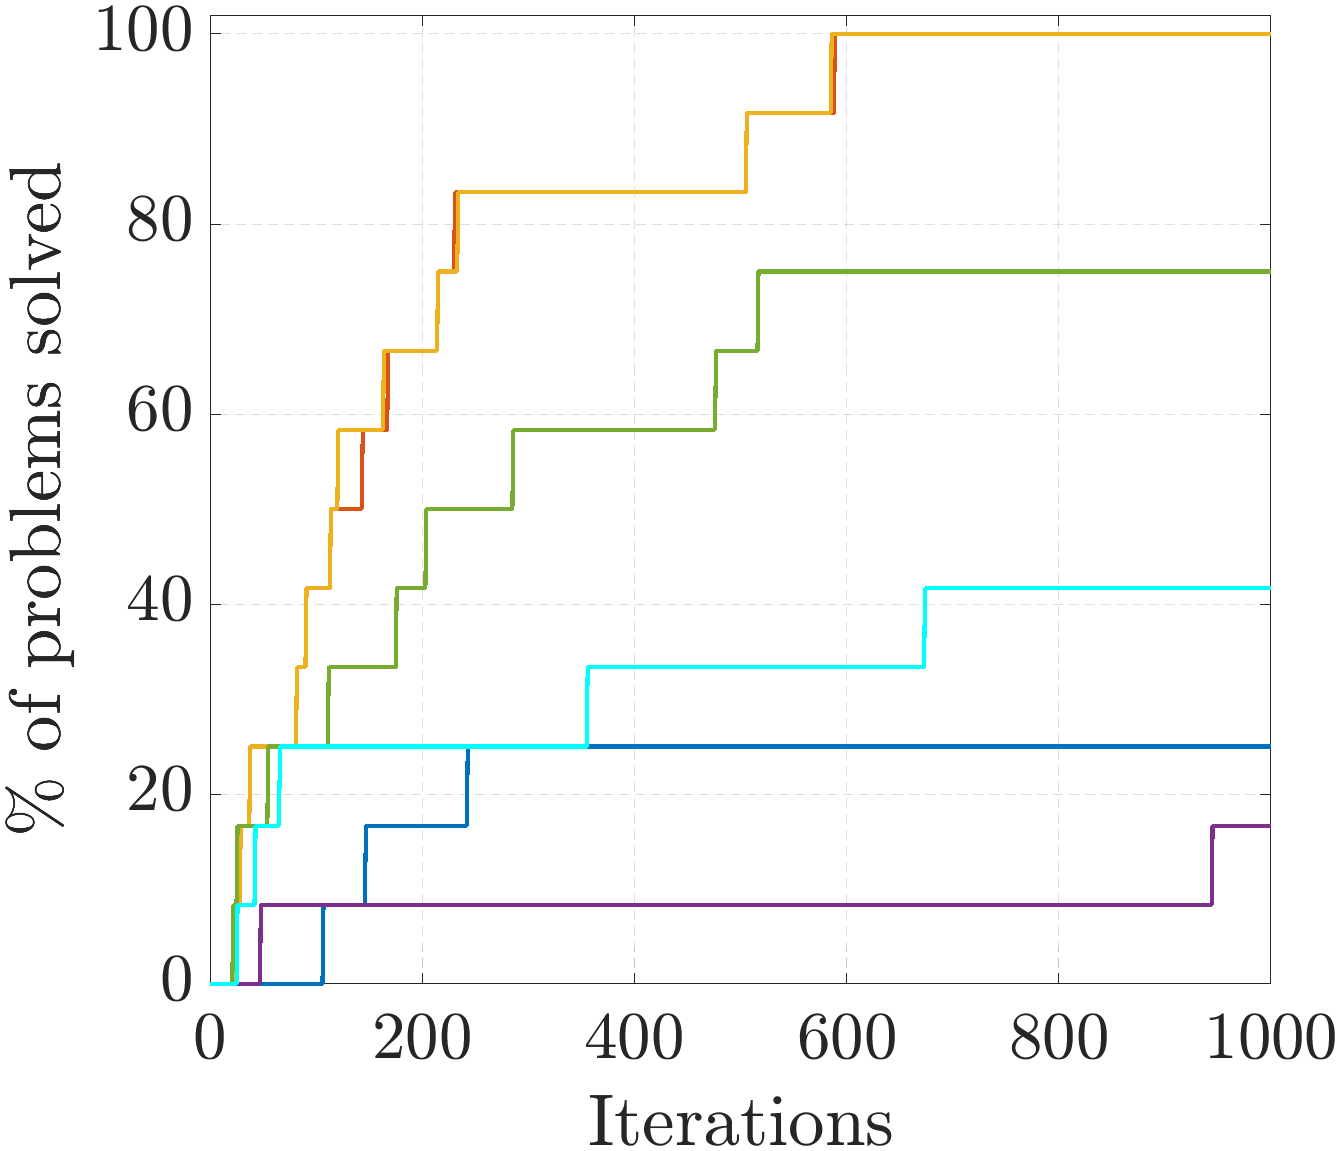
\includegraphics[trim =0mm 0mm 0mm 0mm,width=0.2425\textwidth]{figures/succ/succ_iter_1.png}} &
		\hspace{-0.6em}\subfloat[][$\Delta=5\times10^{-3}$]{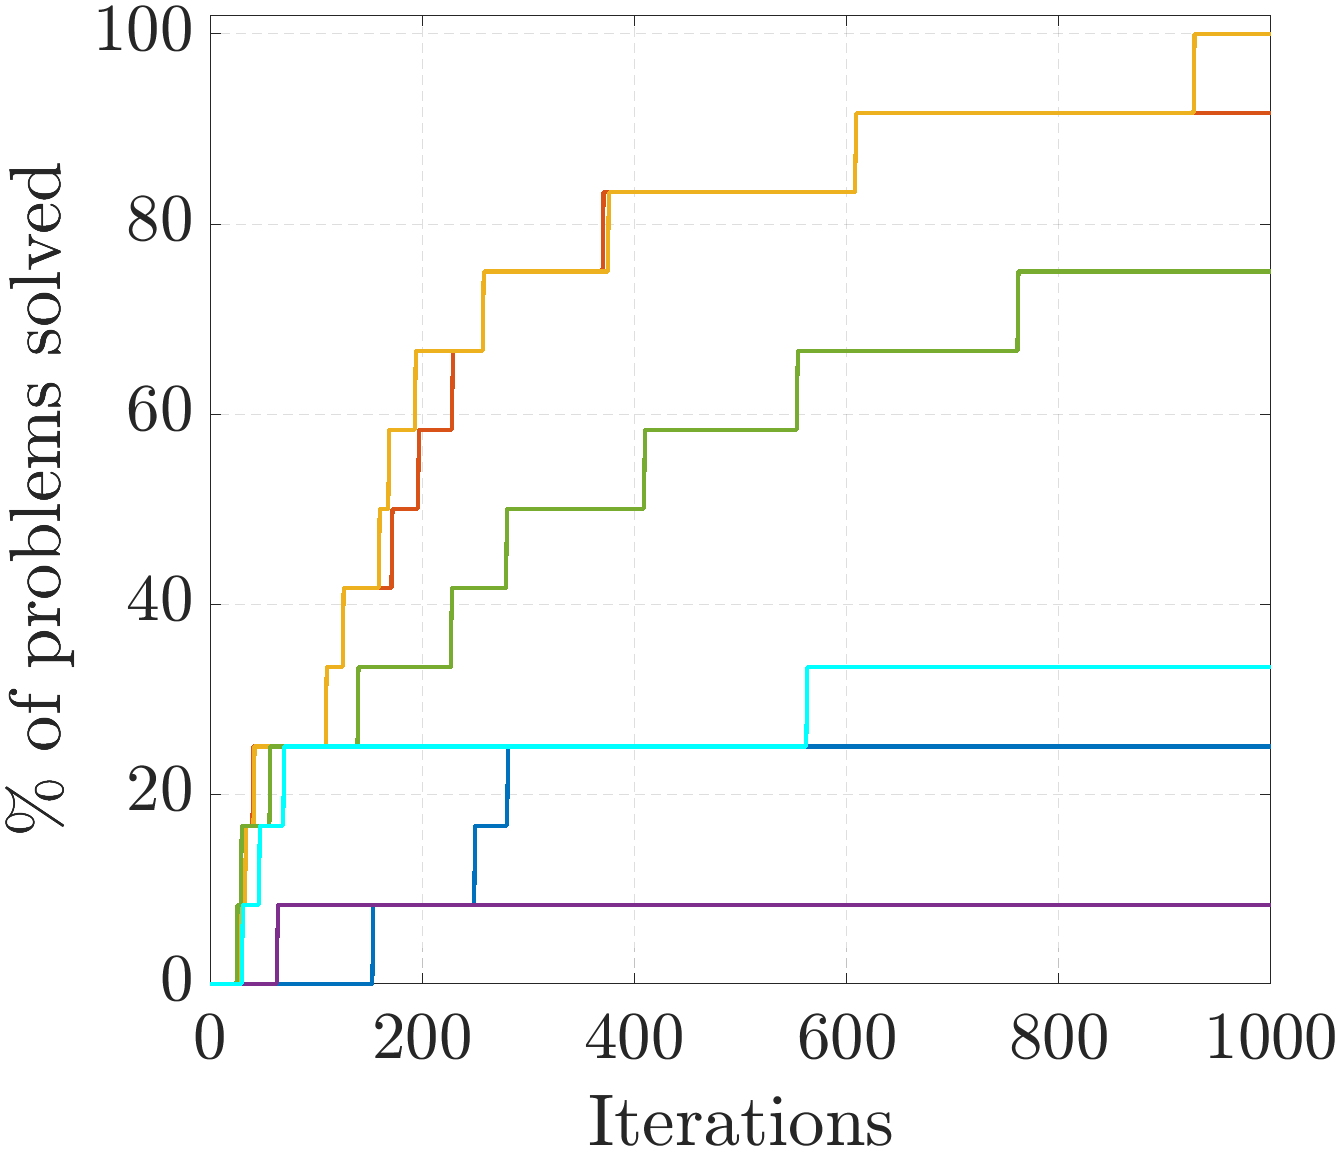
\includegraphics[trim =0mm 0mm 0mm 0mm,width=0.2425\textwidth]{figures/succ/succ_iter_2.png}} &
		\hspace{-0.6em}\subfloat[][$\Delta=1\times10^{-3}$]{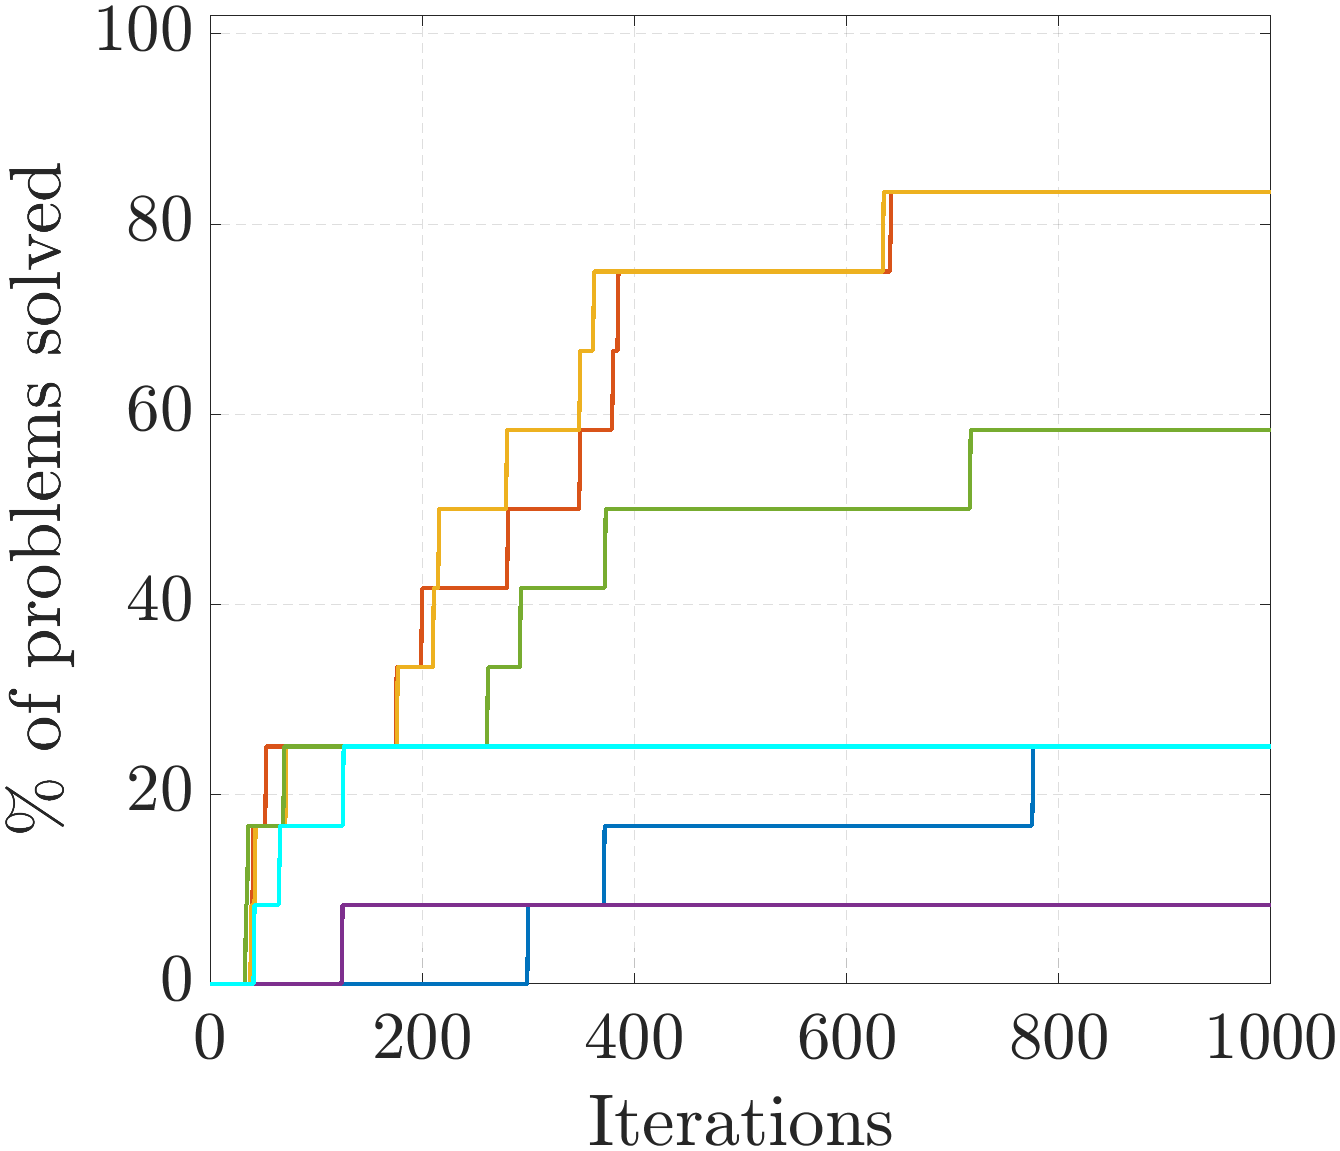
\includegraphics[trim =0mm 0mm 0mm 0mm,width=0.2425\textwidth]{figures/succ/succ_iter_3.png}}&
		\hspace{-0.6em}\subfloat[][$\Delta=1\times10^{-4}$]{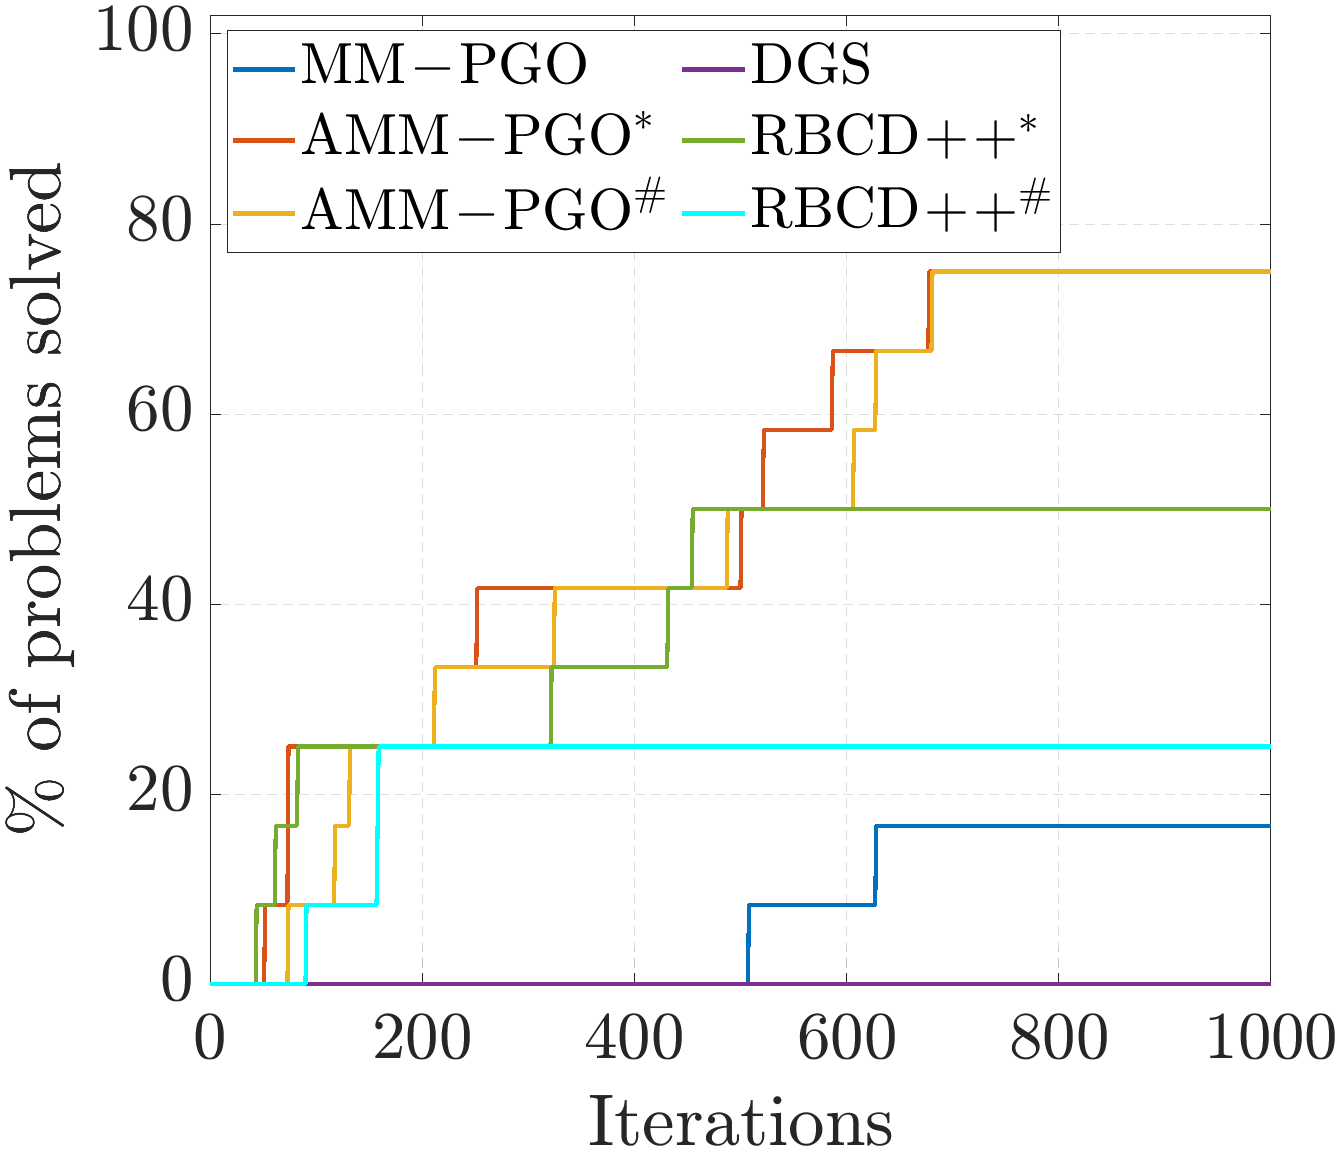
\includegraphics[trim =0mm 0mm 0mm 0mm,width=0.2425\textwidth]{figures/succ/succ_iter_4.png}}
	\end{tabular}
	\caption{Performance profiles for $\mm$, $\ammc$, $\ammd$, $\dgs$ \cite{choudhary2017distributed}, $\rbcdc$ \cite{tian2019distributed} and $\rbcdd$ \cite{tian2019distributed} on 2D and 3D SLAM Benchmark datasets (see \datasetinfo). The performance is based on the number of iterations $\sk$ and the evaluation tolerances are $\Delta=1\times10^{-2}$, $5\times10^{-3}$, $1\times10^{-3}$, $1\times10^{-4}$. The distributed PGO has 10 robots (nodes) and is initialized with distributed Nesterov's accelerated chordal initialization \cite{fan2020mm}. Note that $\ammc$ and $\rbcdc$  require a master node, whereas $\mm$, $\ammd$, $\dgs$  and $\rbcdd$ do not.}\label{fig::succ_iter}
	\vspace{-1em}
\end{figure*}

We also compute the performance profiles \cite{dolan2002benchmarking} based on the number of iterations. Given a  tolerance $\Delta\in(0,\,1]$, the objective value threshold $F_{\Delta}(p)$ of a PGO problem $p$
is 
\vspace{-0.15em}
\begin{equation}\label{eq::Fdel}
F_{\Delta}(p) = F^* + \Delta\cdot\big(F^{(0)}-F^*\big)
\vspace{-0.15em}
\end{equation}
where  $F^{(0)}$ and $F^*$ are the initial and globally optimal objective values, respectively. Let $I_{\Delta}(p)$ denote the minimum number of iterations that  a PGO method takes to reduce the objective value to $F_\Delta(p)$, i.e.,
\vspace{-0.15em}
\begin{equation}
\nonumber
I_{\Delta}(p)\triangleq\min_{\sk}\big\{\sk\geq 0| F^{(\sk)}\leq F_{\Delta}(p)\big\}
\vspace{-0.15em}
\end{equation}
where $F^{(\sk)}$ is the objective value at iteration $\sk$. Then, for a problem set $\mathcal{P}$, the performance profiles of a PGO method is the percentage of problems solved w.r.t. the number of iterations $\sk$:
\vspace{-0.25em}
\begin{equation}
\nonumber
\substack{\text{\normalsize percentage of problems solved}\\ \text{\normalsize at iteration $\sk$}} \triangleq \frac{\big|\{p\in\mathcal{P}|I_{\Delta}(p)\leq \sk\}\big|}{|\mathcal{P}|}.
\end{equation}

The performance profiles based on the number of iterations over a variety of 2D and 3D SLAM benchmark datasets (see \datasetinfo) are shown in \cref{fig::succ_iter}. The tolerances evaluated are $\Delta=1\times10^{-2}$, $5\times10^{-3}$, $1\times10^{-3}$ and $1\times10^{-4}$. We report the performance of $\mm$, $\ammc$, $\ammd$, $\dgs$ \cite{choudhary2017distributed}, $\rbcdc$ \cite{tian2019distributed} and $\rbcdd$ \cite{tian2019distributed} for distributed PGO with 10 robots (nodes). As expected, $\ammc$ and $\ammc$ dominates the other methods ($\mm$, $\dgs$, $\rbcdc$ and $\rbcdd$) in terms of the convergence for all the tolerances $\Delta$, which means that  both of them are better choices for distributed PGO. 


In \cref{table::comp} and \cref{fig::succ_iter}, we emphasize that $\ammd$ requiring no master node achieves comparable performance to that of $\ammc$ using a master node, and is a lot better than all the other methods with a master node ($\rbcdc$) and without ($\mm$, $\dgs$ and $\rbcdd$). Even though $\rbcdc$ and $\rbcdd$ are similarly accelerated with Nesterov's method, we remark that $\rbcdd$ without a master node suffers a great performance drop compared to $\rbcdc$, and more importantly, $\rbcdd$ has no convergence guarantees to first-order critical points. These results reverify that $\ammd$ is more suitable for very large-scale distributed PGO with limited local communication. 

 Note that all of $\mm$, $\ammc$, $\ammd$, $\dgs$ \cite{choudhary2017distributed}, $\rbcdc$ \cite{tian2019distributed} and $\rbcdd$ \cite{tian2019distributed} have to exchange poses of inter-node measurements with the neighbors, and thus, need almost the same amount of communication per iteration. However, \cref{fig::succ_iter} indicates that $\ammc$ and $\ammd$ have much faster convergence in terms of the number of iterations, which also means less communication for the same level of accuracy. In addition, $\rbcdc$ and $\rbcdd$ have to keep part of the nodes in idle during optimization and rely on red-black coloring for block aggregation and random sampling for block selection, which induce additional computation and communication. In contrast, neither $\ammc$ nor $\ammd$ has any extra practical restrictions except \cref{assumption::loss,assumption::mm,assumption::neighbor,assumption::master}.

\begin{figure*}[t]
	\centering
	\begin{tabular}{cccc}
		\hspace{-0.55em}\subfloat[][$\Delta=1\times10^{-2}$]{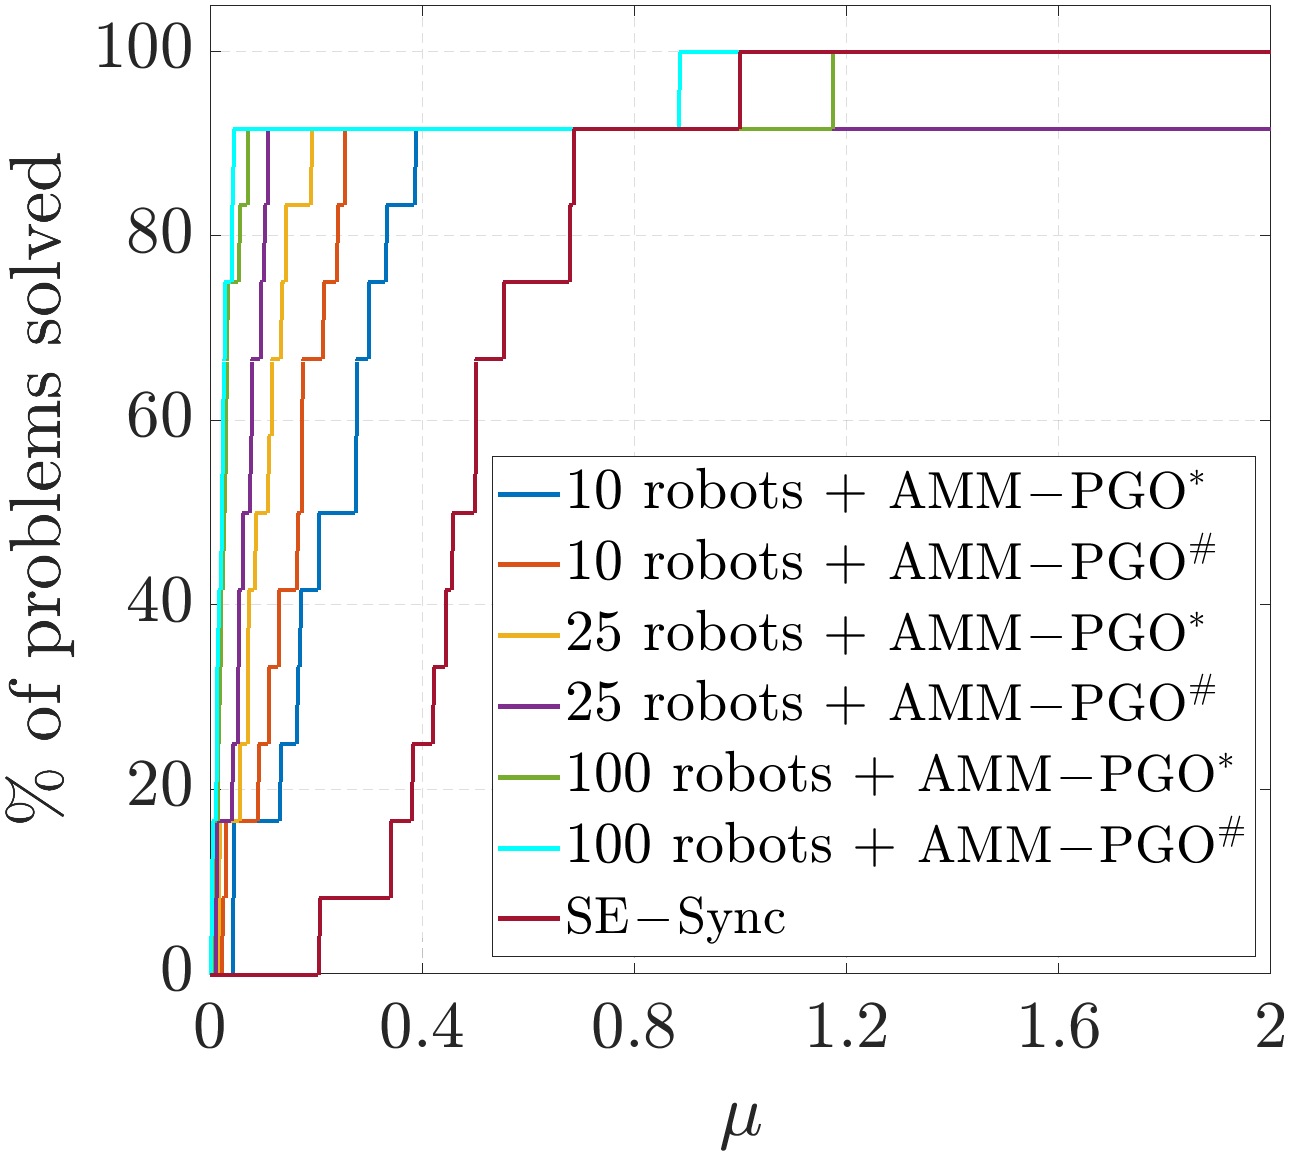
\includegraphics[trim =0mm 0mm 0mm 0mm,width=0.24\textwidth]{figures/succ/succ_time_1.png}} &
		\hspace{-0.55em}\subfloat[][$\Delta=1\times10^{-3}$]{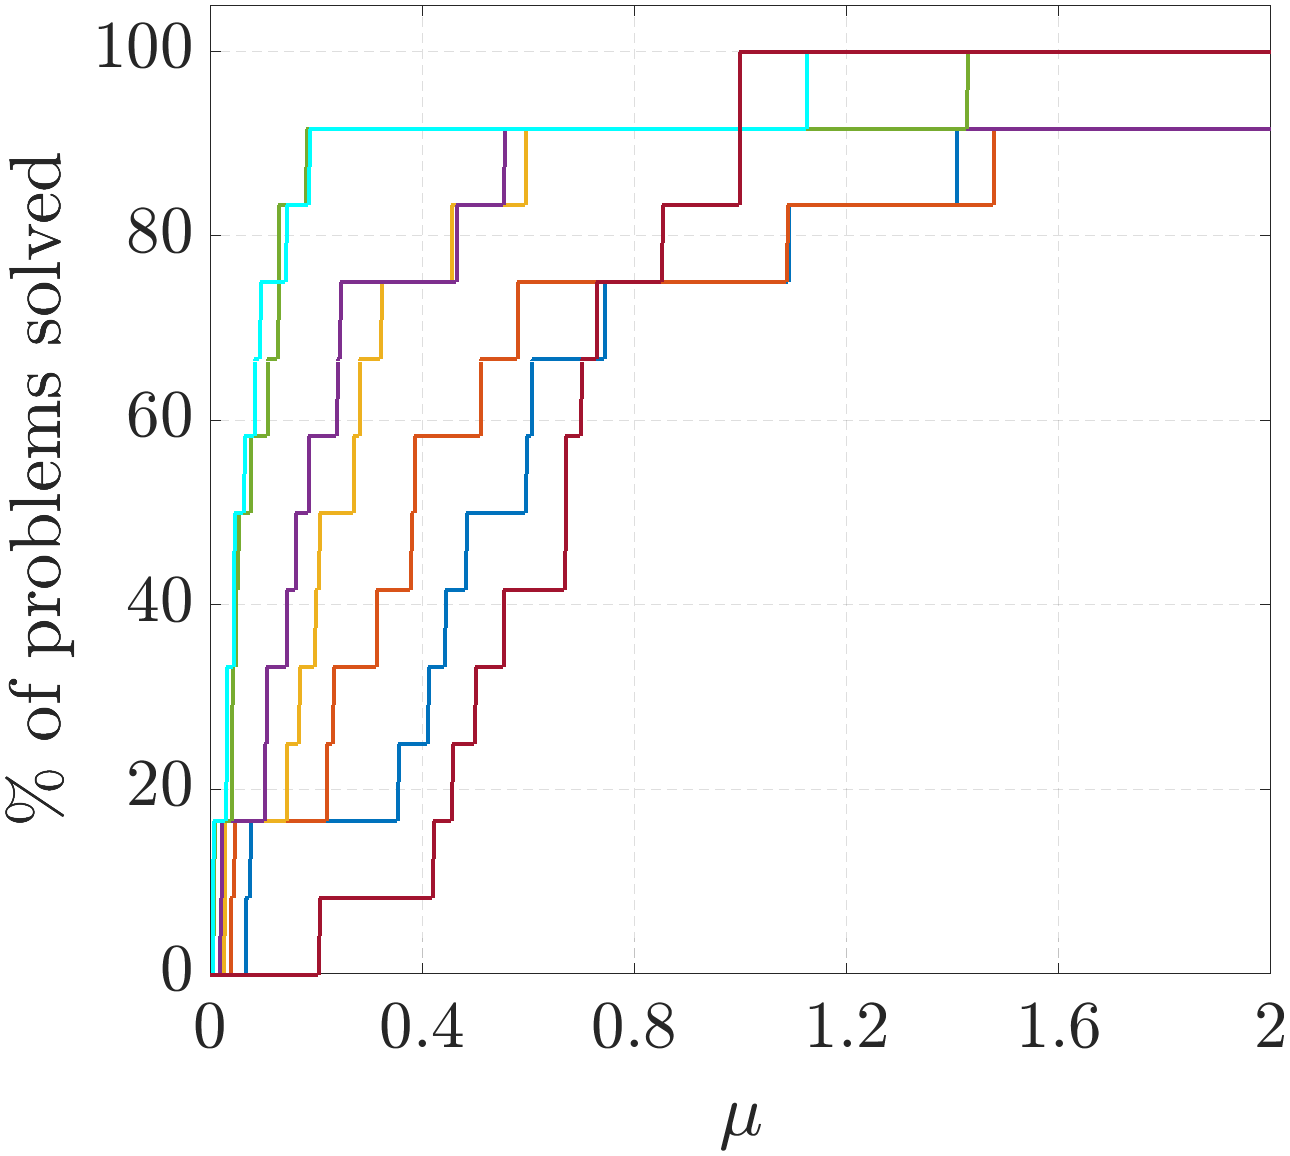
\includegraphics[trim =0mm 0mm 0mm 0mm,width=0.24\textwidth]{figures/succ/succ_time_2.png}} &
		\hspace{-0.55em}\subfloat[][$\Delta=1\times10^{-4}$]{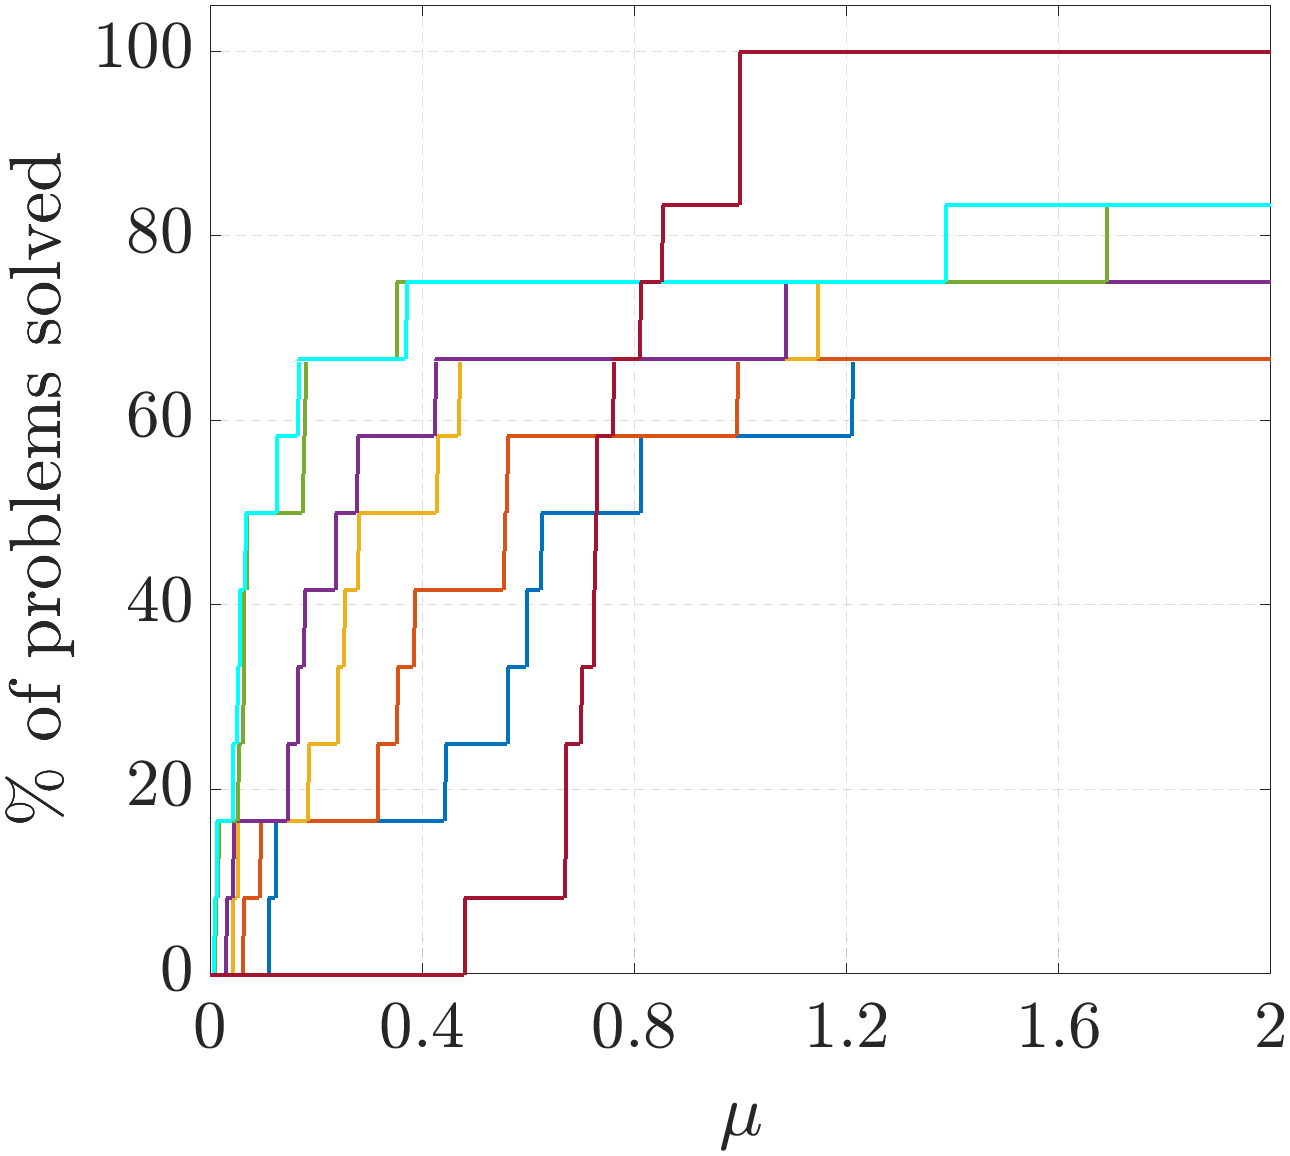
\includegraphics[trim =0mm 0mm 0mm 0mm,width=0.24\textwidth]{figures/succ/succ_time_3.png}}&
		\hspace{-0.55em}\subfloat[][$\Delta=1\times10^{-5}$]{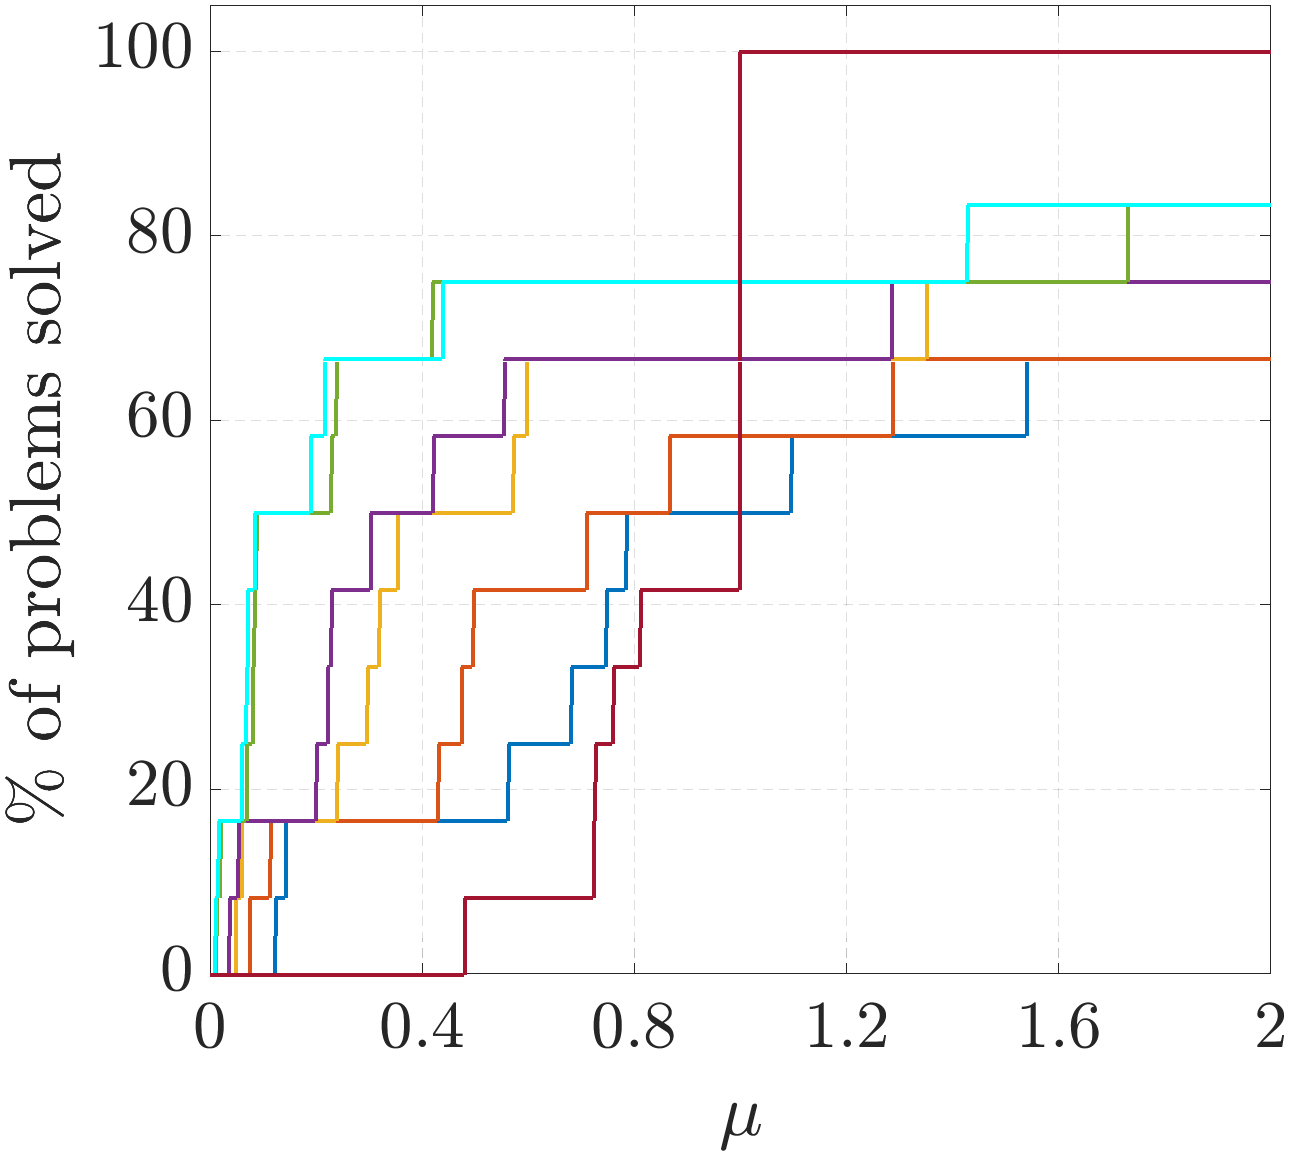
\includegraphics[trim =0mm 0mm 0mm 0mm,width=0.24\textwidth]{figures/succ/succ_time_4.png}}
	\end{tabular}
	\caption{Performance profiles for $\ammc$, $\ammd$ and $\sesync$ \cite{rosen2016se} on 2D and 3D SLAM benchmark datasets (see \datasetinfo). The performance is based on the scaled average optimization time per node $\ratio\in[0,\,+\infty)$ with  tolerances $\Delta=1\times10^{-2}$, $1\times10^{-3}$, $1\times10^{-4}$, $1\times10^{-5}$. The distributed PGO has 10, 25 and 100 robots (nodes) and is initialized with the centralized  chordal initialization \cite{carlone2015initialization}. Note that $\sesync$  solves all the PGO problems globally at $\ratio =1$. }\label{fig::succ_time}
	\vspace{-1.em}
\end{figure*}

\textbf{Optimization Time.} We evaluate the optimization time of $\ammc$ and $\ammd$ with different numbers of robots (nodes) against the centralized baseline $\sesync$ \cite{rosen2016se}. To improve the  time efficiency of our methods, $\Xakp$ in \cref{eq::xG,eq::GYak}  uses the same rotation as $\Xakh$ in \cref{eq::xlG,eq::HYak} and merely updates the translation. Due to the different numbers of robots (nodes), the centralized chordal initialization \cite{carlone2015initialization} is used for all the runs.

Similar to the number of iterations, we use the performance profiles to evaluate $\ammc$ and $\ammd$ in terms of the optimization time. Recall from \cref{eq::Fdel} the objective value threshold $F_{\Delta}(p)$ where $p$ is the PGO problem and $\Delta\in(0,\,1]$ is the tolerance. Since the average optimization time per node is directly related with the speedup, we measure the efficiency of a distributed PGO method with $N$ nodes by computing the average optimization time $T_{\Delta}(p,N)$ that each node takes to reduce the objective value to $F_{\Delta}(p)$:
\vspace{-0.25em}
\begin{equation}\label{eq::TdeltaN}
T_{\Delta}(p,N)=\tfrac{T_\Delta(p)}{N}
\vspace{-0.25em}
\end{equation}
where $T_\Delta(p)$ denotes the total optimization time of all the $N$ nodes. We remark that the centralized optimization method has $N=1$ node and $T_{\Delta}(p,N)=T_{\Delta}(p)$. Let $T_{\sesync}$ denote the optimization time that $\sesync$ needs to find the globally optimal solution. The performance profiles assume a distributed PGO method solves problem $p$  for some $\ratio\in[0,\,+\infty)$ if $T_{\Delta}(p,N)\leq \ratio\cdot T_{\sesync}$. Note that $\ratio$ is the scaled average optimization time per node and $\sesync$ solves problem $p$ globally at $\ratio=1$. 

As a result of \cite{dolan2002benchmarking}, the performance profiles evaluate the speedup of distributed PGO methods for a given optimization problem set $\mathcal{P}$ using  the percentage of problems solved w.r.t. the scaled average optimization time per node $\ratio\in[0,\,+\infty)$: 
\vspace{-0.25em}
\begin{equation}
	\nonumber
	\substack{\text{\normalsize percentage of problems}\\ \text{\normalsize  solved at $\ratio$}} \triangleq\! \frac{\big|\{p\in\mathcal{P}|T_{\Delta}(p,\,N)\!\leq\! \ratio\cdot T_{\sesync}\}\big|}{|\mathcal{P}|}.
\end{equation}
Our method, due to the optimization method taking distribution into account, can be parallelized while retaining guarantees on convergence and computation. A comparison using $T_{\sesync}$ assumes there is no value in parallelization, and indeed in that setting $\sesync$ would be competitive with our method. But parallelization is valuable, and the $T_{\Delta}(p,N)=\tfrac{T_\Delta(p)}{N}$ metric  in \cref{eq::TdeltaN} captures that value, and shows that when we distribute the optimization across agents we get performance that is both superior in accuracy and faster.

\cref{fig::succ_time} shows the performance profiles based on the scaled average optimization time per node. The tolerances evaluated are $\Delta=1\times10^{-2}$, $1\times10^{-3}$, $1\times10^{-4}$ and $1\times10^{-5}$. We report the performance of $\ammc$ and $\ammd$ with $10$, $25$ and $100$ robots (nodes). For reference, we also evaluate the performance profile of the centralized PGO baseline $\sesync$ \cite{rosen2016se}.  As the results demonstrate, $\ammc$ and $\ammd$ are significantly faster than $\sesync$ \cite{rosen2016se} in most cases for modest accuracies of $\Delta=1\times 10^{-2}$ and $\Delta=1\times 10^{-3}$, for which the only challenging case is the {\sf CSAIL} dataset, whose chordal initialization is already very close to the globally optimal solution.  In spite of the performance decline for smaller tolerances of $\Delta=1\times 10^{-4}$ and $\Delta=1\times 10^{-5}$, $\ammc$ and $\ammd$ with 100 robots (nodes) still achieve a $2.5\sim 20\mathrm{x}$ speedup of optimization time over $\sesync$ for more than $70\%$ of the benchmark datasets, not to mention that the average optimization time per node of $\ammc$ and $\ammd$ decreases with the number of robots (nodes). {\highlight Note that the communication overhead is not considered in the experiments.} Nevertheless  \cref{fig::succ_time} indicates that $\ammc$ and $\ammd$ are promising  as fast parallel backends for very large-scale PGO and real-time multi-robot SLAM.


In summary, $\ammc$ and $\ammd$ achieve the state-of-the-art performance for distributed PGO and enjoy a significant multi-node speedup compared to the centralized baseline \cite{rosen2016se} for modestly but sufficiently accurate estimates.

\subsection{Robust Distributed PGO} 

In this section, we evaluate the robustness of $\ammd$ against the outlier inter-node loop closures. Similar to \cite{chang2020kimera,lajoie2020door}, we first use the distributed pairwise consistent measurement set maximization algorithm ($\pcm$) \cite{mangelson2018pairwise} to reject spurious inter-node loop closures and then solve the resulting distributed PGO using $\ammd$ with the trivial, Huber  and Welsch loss kernels in \cref{example::GM,example::trivial,example::huber} . 

We implement $\ammd$ on the 2D {\sf intel} and 3D {\sf garage} datasets (see \datasetinfo) with 10 robots (nodes). For each dataset, we add false inter-node loop closures with uniformly random rotation and translation errors in the range of $[0,\,\pi]$ rad and $[0,\,5]$ m, respectively. In addition, after the initial outlier rejection using the $\pcm$ algorithm \cite{mangelson2018pairwise}, we initialize $\ammd$ with distributed Nesterov's accelerated chordal initialization \cite{fan2020mm} for all the loss kernels. 


The absolute trajectory errors (ATE)  of $\ammd$ w.r.t. different {\highlight outlier ratios} of inter-node loop closures are  in \cref{fig::outlier}. The ATEs are computed against the outlier-free results of $\sesync$ \cite{rosen2016se}  and  averaged over 10 Monte Carlo runs. 

\begin{figure}[t]
	\vspace{-0.75em}
	\centering
	\begin{tabular}{cc}
		\hspace{-0.95em}\subfloat[][{\sf intel}]{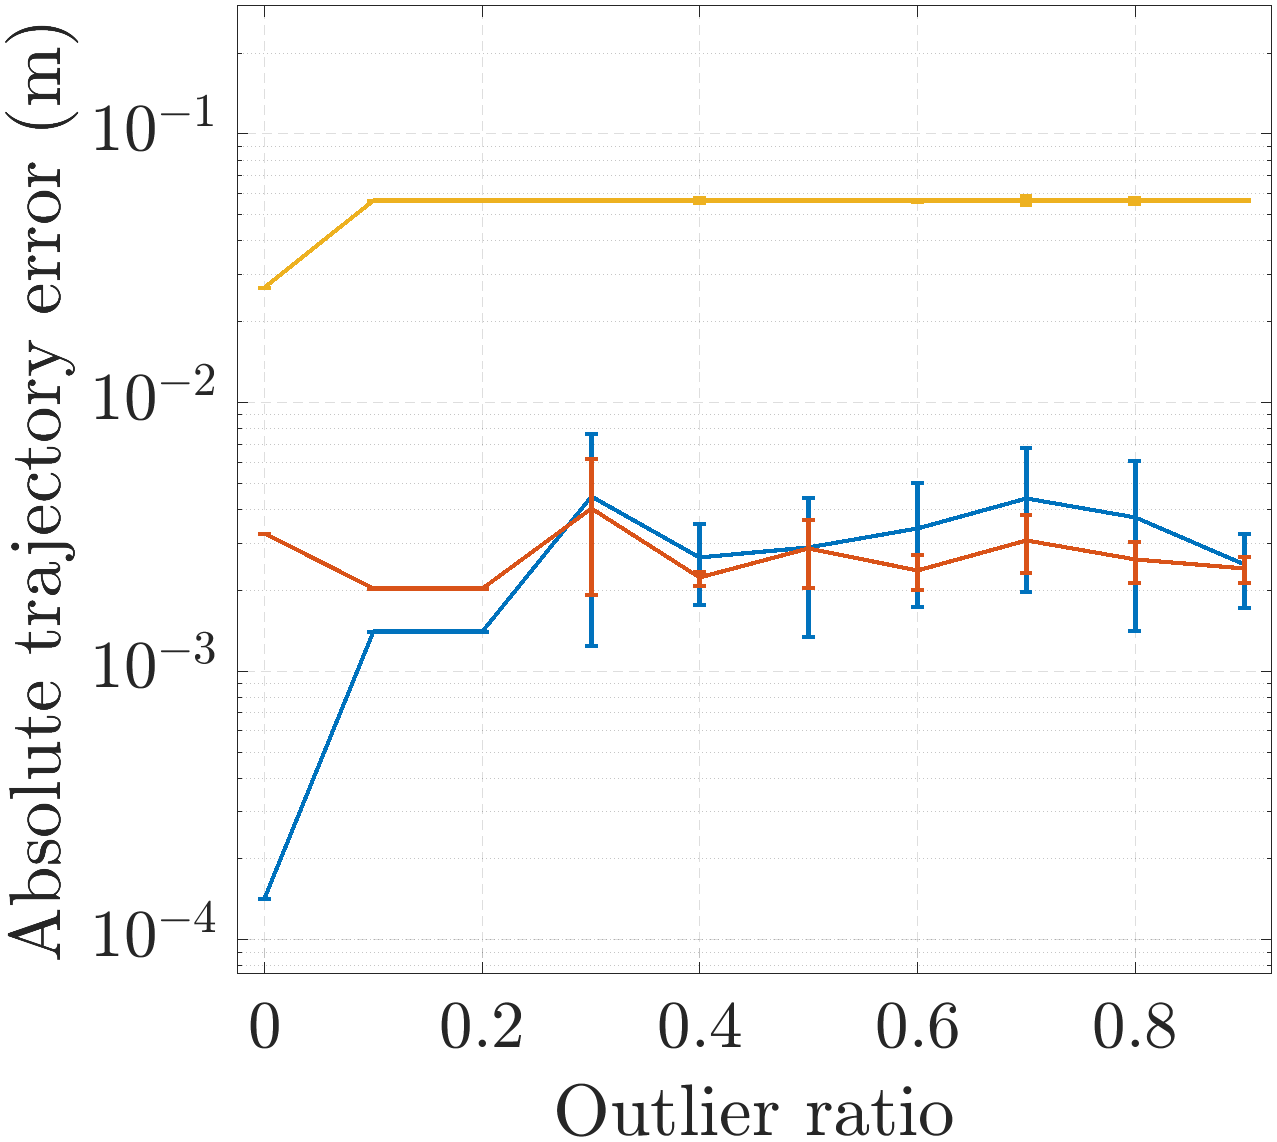
\includegraphics[trim =0mm 0mm 0mm 0mm,width=0.235\textwidth]{figures/outlier/ate_outlier_intel.png}} &
		\hspace{-0.55em}\subfloat[][{\sf garage}]{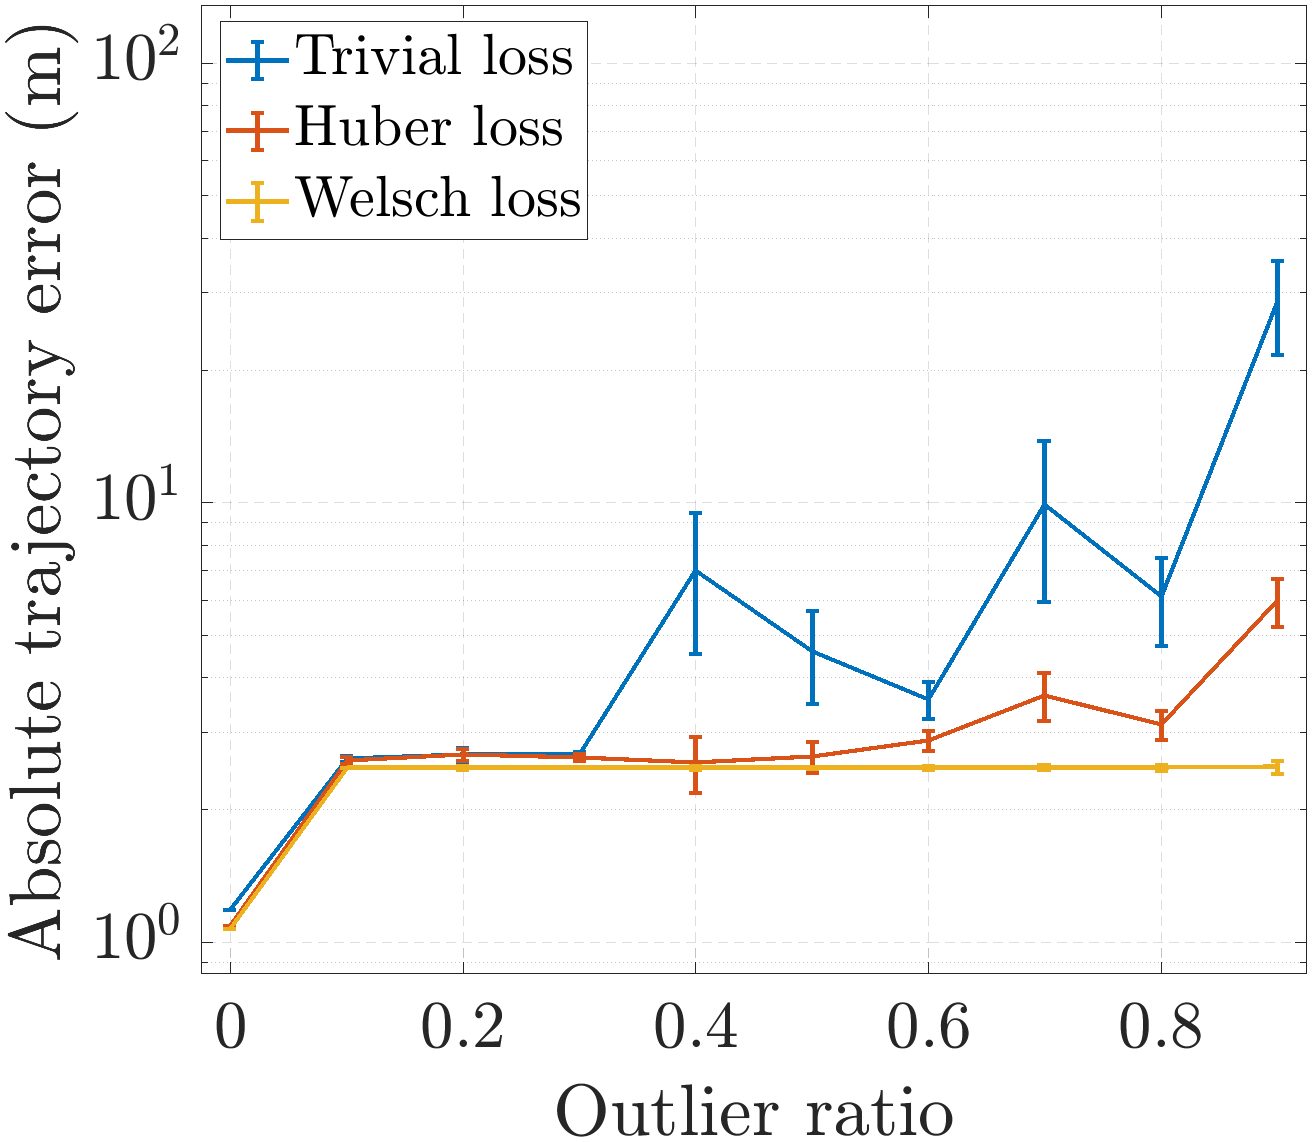
\includegraphics[trim =0mm 0mm 0mm 0mm,width=0.2425\textwidth]{figures/outlier/ate_outlier_garage.png}}
	\end{tabular}
	\caption{Absolute trajectory errors (ATE) of distributed PGO using $\ammd$ with the trivial, Huber and Welsch loss kernels on the 2D {\sf intel} and 3D {\sf garage} datasets.  The {\highlight outlier ratios} of inter-node loop closures are $0\sim 0.9$. The ATEs are computed against the outlier-free results of $\sesync$ \cite{rosen2016se} and  are averaged over $10$ Monte Carlo runs.   $\pcm$  \cite{mangelson2018pairwise} is used to initially reject spurious loop closures.   }\label{fig::outlier}
	\vspace{-.5em}
\end{figure}

In \cref{fig::outlier}(a), $\pcm$ \cite{mangelson2018pairwise} rejects most of the outlier inter-node loop closure for the {\sf intel} dataset and $\ammd$ solves the distributed PGO problems regardless of the loss kernel types and {\highlight outlier ratios}. Note that $\ammd$ with the Welsch loss kernel has larger ATEs (avg. $0.057$ m) against $\sesync$ \cite{rosen2016se} than those with the trivial and Huber loss kernels (avg. $0.003$ m), and we argue that this is related to the loss kernel types. The ATEs are evaluated based on $\sesync$ using the trivial loss kernel, which is in fact identical/similar to distributed PGO with the trivial and Huber loss kernels but different from that with the Welsch loss kernel. Thus, the estimates from the trivial and Huber loss kernels are expected to be more close to those of $\sesync$, which result in smaller ATEs compared to the Welsch loss kernel  if no outliers.

\figgarage

For the more challenging {\sf garage} dataset, as is shown in \cref{fig::outlier}(b), $\pcm$ fails for {\highlight outlier ratios} over $0.4$, and further, distributed PGO with the trivial and Huber loss kernels results in ATEs as large as $65$ m. In contrast, distributed PGO with the Welsch loss kernel still successfully estimates the poses with an average ATE of $2.5$ m despite the existence of  outliers---note that the {\sf garage} dataset has a trajectory over $7$ km. For the {\sf garage} dataset, a qualitative comparison of distributed PGO with different loss kernels is also presented in \refgarage, where the Welsch loss kernel still has the best performance. The results are not surprising since the Welsch loss kernel is known to be more robust against outliers than the other two loss kernels \cite{barron2019cvpr}.  



The results above indicate that our MM methods can be applied to distributed PGO in the presence of outlier inter-node loop closures when combined with robust loss kernels like Welsch and other outlier rejection techniques like $\pcm$ \cite{mangelson2018pairwise}. In addition, we emphasize again that our MM methods have provable convergence to first-order critical points for a broad class of robust loss kernels, whereas the convergence guarantees of existing distributed PGO methods \cite{choudhary2017distributed,tian2019distributed,tron2014distributed,eric2020geod} are restricted to the trivial loss kernel.